% Template for MSc final reports
% EEE Department - Imperial College London
%
% INSTRUCTIONS
% (1) Compile using LuaLatex (it is the successor of pdflatex). To check this on Overleaf, click on the Menu on the top left.
% (2) Complete the SETUP below

%%%%%%%%%%%%%%%%%%%%%%%%%%%%%%%%%%%%%%%
% DO NOT MODIFY FROM HERE ...
\documentclass[12pt,twosided]{ic_eee_thesis}

\usepackage[style=ieee,backend=biber,hyperref=auto]{biblatex}
\addbibresource{references.bib}
% ... TO HERE
%%%%%%%%%%%%%%%%%%%%%%%%%%%%%%%%%%%%%%%


%%%%%%%%%%%%%%%% SETUP %%%%%%%%%%%%%%%%
%%%%%%%%%%%%%%%%%%%%%%%%%%%%%%%%%%%%%%%
% EDIT THE FOLLOWING INFORMATION WITH YOUR DATA
\title{Algorithmic trading using optimal control in the Julia programming language}
\subtitle{} % use \subtitle{} to remove it
\author{B. Castro}
\cid{02353208}
\supervisor{Prof. E. Kerrigan} %UK: Dr no dot, prof has dot
\submityear{2023}
% PICK A DEGREE FROM THE LIST BELOW 
% DO NOT MODIFY THE NAMES
\course{Control and Optimisation}
%\course{Analogue and Digital Integrated Circuit Design}
%\course{Applied Machine Learning}
%\course{Communications and Signal Processing}
%\course{Control and Optimisation}
%\course{Future Power Networks}

% Do you want a list of figures?
% Do you want a list of tables?
% Do you want an acknowledgement page?
% Do you want a list of acronyms?
\setboolean{list_of_figures}{true} % false or true - Default is true
\setboolean{list_of_tables}{false} % false or true - Default is false
\setboolean{acknowledgement}{true} % false or true - Default is true
\setboolean{acronyms}{true} % false or true - Default is true

%%%%%%%%%%%%% END SETUP %%%%%%%%%%%%%%%
%%%%%%%%%%%%%%%%%%%%%%%%%%%%%%%%%%%%%%%


% ADDITIONAL PACKAGES
% You can add your packages below. Note that the following packages are already loaded: pgfcore, geometry, bookmark, graphicx, setspace, kantlipsum, fontspec, polygrossia (default English), minitoc, silence, background, xpatch, tikzpagenodes, totcount, fancyhdr, titlesec and the tikz libraries calc, shapes.symbols and shapes.misc  

%Examples
\usepackage{caption}
\usepackage{subcaption}
\usepackage{amsmath}
\usepackage{amsfonts}
\usepackage[inkscapelatex=false]{svg}
\usepackage{dsfont}
\usepackage{listings}
\usepackage{xcolor}
\usepackage{algorithm}
\usepackage{algpseudocode}
\usepackage{longtable}
%...

% ADDITIONAL COMMANDS
%Examples
\definecolor{codegreen}{rgb}{0,0.6,0}
\definecolor{codegray}{rgb}{0.5,0.5,0.5}
\definecolor{codepurple}{rgb}{0.58,0,0.82}
\definecolor{mygreen}{RGB}{28,172,0} 
\definecolor{mylilas}{RGB}{170,55,241}
\definecolor{backcolour}{rgb}{0.95,0.95,0.92}

\lstdefinelanguage{Julia}%
  {morekeywords={abstract,break,case,catch,const,continue,do,else,elseif,%
      end,export,false,for,function,immutable,import,importall,if,in,%
      macro,module,otherwise,quote,return,switch,true,try,type,typealias,%
      using,while},%
   sensitive=true,%
   % alsoother={$},%
   morecomment=[l]\#,%
   morecomment=[n]{\#=}{=\#},%
   morestring=[s]{"}{"},%
   morestring=[m]{'}{'},%
}[keywords,comments,strings]%

\lstdefinestyle{JuliaStyle}{
    basicstyle= \ttfamily,
    backgroundcolor=\color{backcolour},   
    commentstyle= \color{ForestGreen},
    keywordstyle=\color{blue},
    numberstyle=\tiny\color{codegray},
    stringstyle=\color{magenta},
    basicstyle=\ttfamily\scriptsize,
    breakatwhitespace=false,         
    breaklines=true,                 
    captionpos=b,                    
    keepspaces=true,                 
    numbers=left,                    
    numbersep=5pt,                  
    showspaces=false,                
    showstringspaces=false,
    showtabs=false,                  
    tabsize=2,
    aboveskip=\medskipamount
}

\lstset{%
    style            = JuliaStyle,
    language         = Julia
}

% \DeclareMathOperator{\diag}{diag}
% \DeclareMathOperator{\vect}{vec}



%\newcommand*{\point}[1]{\vec{\mkern0mu#1}}
\newcommand{\ci}[0]{\perp\!\!\!\!\!\perp} % conditional independence
\newcommand{\point}[1]{{#1}} % points 
\renewcommand{\vec}[1]{{\boldsymbol{{#1}}}} % vector
\newcommand{\mat}[1]{{\boldsymbol{{#1}}}} % matrix
\newcommand{\Normal}[1]{\mathcal{N}(\mu_{#1},\Sigma_{#1})} % Normal Distribution
\newcommand{\D}[0]{\mathcal{D}} % Distribution 
\newcommand{\R}[0]{\mathds{R}} % real numbers

\newcommand{\E}[0]{\mathds{E}} % Expected value
\newcommand{\LL}[0]{\mathcal{L}} % Expected value


\newcommand{\M}[0]{\mathscr{M}} % Model Symbol (Cursive M)

\newcommand{\Z}[0]{\mathds{Z}} % integers
\newcommand{\N}[0]{\mathds{N}} % natural numbers
\newcommand{\nat}[0]{\mathds{N}} % natural numbers
\newcommand{\Q}[0]{\mathds{Q}} % rational numbers
\ifxetex
\newcommand{\C}[0]{\mathds{C}} % complex numbers
\else
\newcommand{\C}[0]{\mathds{C}} % complex numbers
\fi
\newcommand{\tr}[0]{\text{tr}} % trace
\renewcommand{\d}[0]{\mathrm{d}} % total derivative
\newcommand{\inv}{^{-1}} % inverse
\newcommand{\id}{\mathrm{id}} % identity mapping
\renewcommand{\dim}{\mathrm{dim}} % dimension
\newcommand{\rank}[0]{\mathrm{rk}} % rank
\newcommand{\determ}[1]{\mathrm{det}(#1)} % determinant
\newcommand{\scp}[2]{\langle #1 , #2 \rangle}
\newcommand{\kernel}[0]{\mathrm{ker}} % kernel/nullspace
\newcommand{\img}[0]{\mathrm{Im}} % image
\newcommand{\idx}[1]{{(#1)}}
\DeclareMathOperator*{\diag}{diag}

\newcommand{\var}{\mathds{V}} % variance
\newcommand{\gauss}[2]{\mathcal{N}\big(#1,\,#2\big)} % gaussian distribution N(.,.)
\newcommand{\gaussx}[3]{\mathcal{N}\big(#1\,|\,#2,\,#3\big)} % gaussian distribution N(.|.,.)
\newcommand{\gaussBig}[2]{\mathcal{N}\left(#1,\,#2\right)} % see above, but with brackets that adjust to the height of the arguments
\newcommand{\gaussxBig}[3]{\mathcal{N}\left(#1\,|\,#2,\,#3\right)} % see above, but with brackets that adjust to the height of the arguments
\DeclareMathOperator{\cov}{Cov} % covariance (matrix) 

% matrix determinant
\newcommand{\matdet}[1]{
\left|
\begin{matrix}
#1
\end{matrix}
\right|
}


\newcommand{\cw}{4 cm} % Column Width

%%% various color definitions
\definecolor{darkgreen}{rgb}{0,0.6,0}

\newcommand{\blue}[1]{{\color{blue}#1}}
\newcommand{\red}[1]{{\color{red}#1}}
\newcommand{\green}[1]{{\color{darkgreen}#1}}
\newcommand{\orange}[1]{{\color{orange}#1}}
\newcommand{\magenta}[1]{{\color{magenta}#1}}
\newcommand{\cyan}[1]{{\color{cyan}#1}}

\newcommand\hcancel[2][black]{\setbox0=\hbox{$#2$}%
\rlap{\raisebox{.45\ht0}{\textcolor{#1}{\rule{\wd0}{1pt}}}}#2} 

\newcommand{\st}[1]{{\hcancel[red]{#1}}}

% redefine emph
\renewcommand{\emph}[1]{\blue{\bf{#1}}}

% place a colored box around a character
\gdef\colchar#1#2{%
  \tikz[baseline]{%
  \node[anchor=base,inner sep=2pt,outer sep=0pt,fill = #2!20] {#1};
    }%
}%
 % short-hand notation and macros

%...


\begin{document}

\preamble % Do not change - required

% EDIT THE CONTENT OF THE FILES
% Abstract.tex
% OrigSta_Copyright.tex
% Acknowledgement.tex
% You can find them under the folder 
% "chapters" on the left column

% ADD AS MANY CHAPTERS AS NEEDED
% BY CREATING .TEX FILES IN THE FOLDER chapters
% AND ADDING \input{namechapter.tex} BELOW
\chapter{Introduction}
\label{ch1}

\adjustmtc % Adjust Minitoc to right chapter
%%%%%%%%%%%%%%%%%%%%%%%%%%%%%%%%%%%%%%%
% IMPORTANT
\singlespacing % THESE THREE
\minitoc % LINES MUST APPEAR IN
\doublespacing % EVERY CHAPTER
% COPY THEM IN ANY NEW CHAPTER
%%%%%%%%%%%%%%%%%%%%%%%%%%%%%%%%%%%%%%%


\section{Project Introduction}
This project presents general framework for Algorithmic trading native to Julia, capable of solving portfolio optimization problems using \ac{MPC}, called AirBorne. 

In particular, in Chapter \ref{ch5}, AirBorne will be used as the simulation framework running a state of the art \ac{MPC} that uses \ac{HMM} in combination with a Mean-Variance framework to estimate an optimal portfolio distribution over time that maximizes a balance between expected returns and the variance of the return.

In Chapter \ref{ch1} and introduction to the project, its motivation and related works are addressed. Chapter \ref{ch2} introduces necessary concepts for Financial modelling that be linked to the dynamics of the system.  Chapter \ref{ch3} addresses the \ac{OCP} formulation and introduces the \ac{MPC} model.  Chapter \ref{ch4} addresses the design of AirBorne and identifies some unique traits of the Julia language leveraged on the project. Lastly Chapter \ref{ch5} presents results of the implementation of multiple trading strategies using AirBorne as the framework for the simulations.

\subsection{Motivation}

Portfolio optimization and algorithmic trading is an active area of research in all fields from mathematical formulations \cite{RL2022,2022OptimalControl} to ethics and law  \cite{ethicsAndLaw2022}, whilst some algorithms are reported to outperform human traders on normal circumstances on complex market conditions humans still have the edge \cite{algorithmicTradingWithHumanTraders}. In recent years control theory techniques such as \ac{MPC} are being increasingly used for portfolio optimization, formulating the management of assets as a control problem \cite{MultiPeriod_PO_mpc}. 

At the same time Julia, a relatively new language, often compared to Python on its expressiveness and C on its performance, lacks well developed and maintained packages suitable for algorithmic trading and backtesting hindering its potential and adoption rate for algorithmic trading purposes \cite{juliaReview2021}. 

Therefore the aim of this project is to produce software native to Julia for portfolio optimization and algorithmic trading simulation to accelerate research in the future in the area and this language. 

\subsection{Related work}

Many groups in Github have tried to deploy similar software in the past, most of the attempts resulted in projects with great initial development but died out eventually due to lack of continuous support and maintenance. Some of the most prominent related projects are:

\begin{enumerate}
    \item \textbf{JuliaQuant:} They tried to provide an ecosystem of algorithmic trading tools from analysis to model of portfolios. Although they have been around for more than 5 years the intensity of development has winded down significantly, having their last commit to any of their repositories to January 2023, \url{https://github.com/JuliaQuant}. 
    \item \textbf{Julia Finance:} Also following a similar approach to JuliaQuant they provided different models of entities such like assets and currencies. Most of the repositories are not actively maintained with the exception of ``BusinessDays", \url{https://github.com/JuliaFinance}.
    \item \textbf{Trading.jl:} This is a single package focused on designing tools for back-testing, is a relatively young package and although promising it being supported by a single person poses a key-person risk.\url{https://github.com/louisponet/Trading.jl}
\end{enumerate}

All these previous attempts have in common to be maintained by a handful of individuals, with a sharp fast initial development and subsequent slower development pace. 

AirBorne has the advantage of being institutionally backed by Imperial College London, ensuring its support and maintenance as long as the project is deemed relevant by their leaders, this ensures renewal of people for its support and continuous improvement until it has features rich enough for the community to adopt it and evolve into a community maintained open-source package.

This approach similar to python starts the package being institutionally backed on its early stages were continuous support and improvement are critical for the development of the package until is of enough value for the community to adopt, nourish and maintain, such as the Python and C++ AirBorne counterparts Zipline and Zorro projects.


\subsubsection{Julia package ecosystem}
In Julia is important to design software packages compatible with other related and used packages, which is commonly known as the ecosystem of a package. Some of the packages AirBorne's ecosystem are:
\begin{enumerate}
    \item \textbf{ValueAtRisk.jl:} Package specialized in calculated the \ac{VaR} metric.
    \item \textbf{Currencies.jl:} Alternative package for currency modelling complying with ISO guidelines.
    \item \textbf{ARCHModels.jl:} Produces ARCH models. ARCH models are variants of ARMAX models widely used in financial applications such as inflation simulation with seasonal volatility \cite{ARCHModels.jl,Periodic_ARCHModels_og_paper,ARCHModels_og_paper}.
    \item \textbf{DirectSearch.jl: } A package developed by Imperial College London, which implements the optimization algorithm \ac{MADS}\cite{DirectSearch.jl,MADS_og_paper_06}. It  derivative free optimization algorithm, ideal for empirically driven optimization problems where a descent direction may not be available or hard to deduce.
\end{enumerate}

\subsubsection{Past research projects}

In recent years Imperial students have tried many formulations to address advisory algorithmic trading, were a computer suggest trading strategies to a human prior to execution. Some techniques used were Reinforcement Learning  \cite{RLMasoud2021}, Behavioural Control Theory  \cite{BCTScott2022,BCTKhaliq2022} and Data Enabled Predictive Control \cite{DeePCMohamed2023}.

Although many of these projects achieved a stand alone implementation of portfolio optimization they didn't produce a general software capable of implementing custom trading strategies and be able to compare and analyze them. 

This project will build on top of their work and create a generalized framework to benchmark and compare different techniques for portfolio optimization in the Julia programming language along with an implementation using Optimal Control.


\section{Introduction AirBorne}
Chapter \ref{ch2} introduces the theoretical background for the algorithmic trading problem but also establishes some links between the theory and the design of the software. Therefore an overall introduction to the \ac{HLD} of AirBorne will be presented here and justified through Chapters \ref{ch2} and \ref{ch4}.

\begin{figure}[h!]
    \centering
    % \includesvg[width=1\textwidth]{imgs/ch1/SoftwareArchitecture.svg}
    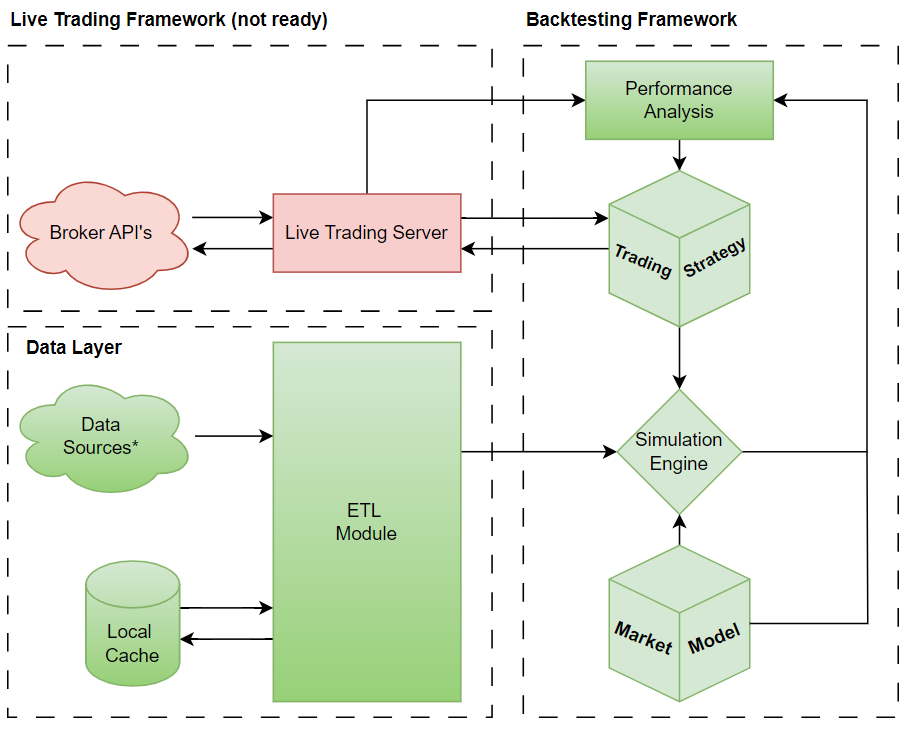
\includegraphics[width=1\textwidth]{imgs/ch1/architecture.png}
    \caption[AirBorne: Overall Architecture]{AirBorne: Overall Architecture}
    \label{fig::AirBorneArchitecture}
\end{figure}

Figure \ref{fig::AirBorneArchitecture} shows the overall architecture of AirBorne, which is composed of three components:
\begin{enumerate}
    \item \textbf{Data Layer:} Where connections to data sources, local storage in persisted memory (the cache) and common data manipulation take place.
    \item \textbf{Backtesting Framework:} Where simulations take place and trading strategies, models for markets and performance calculations are defined.
    \item \textbf{Live Trading Framework:} This layer provides an interface with brokerage accounts and broker \ac{API}s, allowing to switch a trading strategy from simulation to live or paper trading seamlessly. 
\end{enumerate}

Of these three components, for the project the Backtesting Framework and Data Layer were developed, and the implementation of the Live Trading Framework was left out from the scope of the project.

Figure \ref{fig::AirBorneModules} shows the hierarchy of submodules, where the higher submodules have some dependency or are supported by the lower ones.

\begin{figure}[h!]
    \centering
    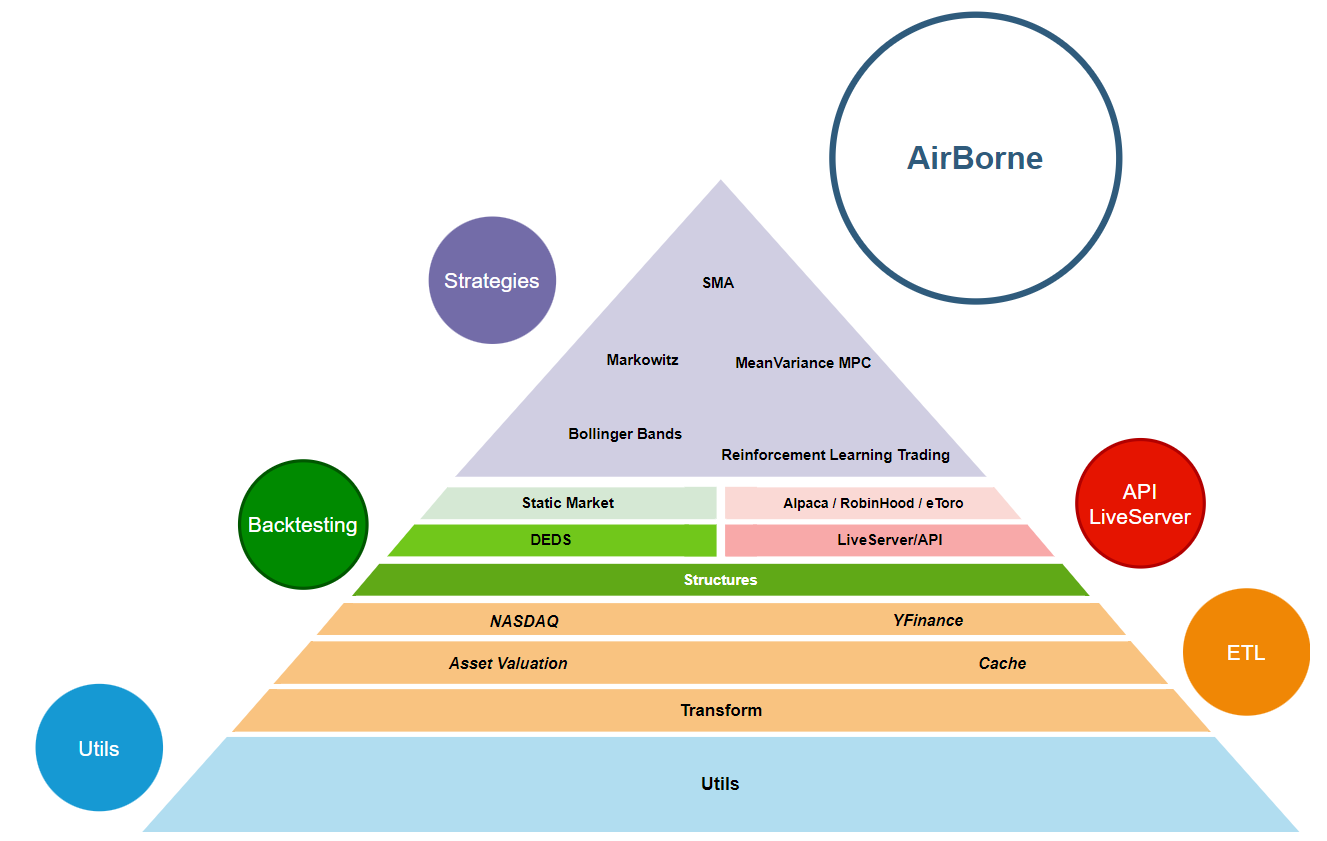
\includegraphics[width=1\textwidth]{imgs/ch1/Hierarchy.png}
    \caption[AirBorne: Module Hierarchy]{AirBorne: Module Hierarchy}
    \label{fig::AirBorneModules}
\end{figure}

\textbf{Utils} contains basic functions used throughout the module, this reduces duplicate code throughout, \textbf{ETL} provides the tools for data handling and storage of data in the system that can be processed during the simulation or backtesting stages. Then the pyramid branches into \textbf{Backtesting} and \textbf{Live Trading}, both of this layers share common data structures, but one specializes in simulation/modelling of the market whilst the second one provides direct connection to the real market. Lastly \textbf{Strategies} produces investment strategies that are designed to be incorporated either on backtesting or live-trading instances.


\section{Notation}

Standard notation has been adopted in the Thesis, most of which is defined in this section and used throughout the remainder of the Thesis. When new notation, not included in this section is introduced, this is defined in the relevant parts of the Thesis.\smallskip\\

\begin{enumerate}
    \item $\delta_{\odot}$: Delta Kronecker applied to each entry of an array
    \item $\odot$: Element wise product
\end{enumerate}

% \indent The symbol $\mathbb{R}_{\ge0}$ ($\mathbb{R}_{>0}$) denotes the set of non-negative (positive) real numbers; $\mathbb{C}_{<0}$ denotes the set of complex numbers with strictly negative real part; $\mathbb{C}_{0}$ denotes the set of complex numbers with zero real part and $\mathbb{D}_{<1}$ the set of complex numbers with modulo less than one.\smallskip\\
% \indent The symbol $I$ denotes the identity matrix and $\sigma(A)$ denotes the spectrum of the matrix $A\in\mathbb{R}^{n\times n}$. The symbol $\otimes$ indicates the Kronecker product and $||A||$ indicates the induced Euclidean matrix norm. Given a list of $n$ elements $a_i$, $\diag(a_i)$ indicates a diagonal matrix with diagonal elements equal to the $a_i$'s. The vectorization of a matrix $A\in\mathbb{R}^{n\times m}$, denoted by $\vect(A)$, is the $nm \times 1$ vector obtained by stacking the columns of the matrix $A$ one on top of the other, namely $\vect(A)=[a_1^{\top},a_2^{\top},\dots,a_m^{\top}]^{\top}$, where $a_i\in\mathbb{R}^n$ are the columns of $A$ and the superscript $\top$ denotes the transposition operator. The superscript $*$ indicates the conjugate transpose operator.\smallskip\\
% \indent The symbol $\Re[z]$ indicates the real part of the complex number $z$, $\Im[z]$ denotes its imaginary part and $\iota$ denotes the imaginary unit. The symbol $\epsilon_k$ indicates a vector with the $k$-th element equal to 1 and with all the other elements equal to 0. Given a function $f$, $\overline{F}$ represents its phasor at $\omega$, whereas $<\!f(t)\!>$ indicates its time average.\smallskip\\
% \indent Given a set of delays $\{\tau_j\}$, the symbol $\mathfrak{R}_T^n=\mathfrak{R}_T^n([-T,0],\mathbb{R}^n)$, with $T=  \max_j\{\tau_j\}$, indicates the set of continuous functions mapping the interval $[-T,0]$ into $\mathbb{R}^n$ with the topology of uniform convergence . The subscripts ``$\tau_j$'' and ``$\chi_j$'' denote the translation operator, \textit{e.g.}\ $x_{\tau_j}(t)=x(t-\tau_j)$.\smallskip\\
% \indent Let $\bar s \in \mathbb{C}$ and $A(s)\in \mathbb{C}^{n \times n}$. Then $\bar s\notin\sigma(A(s))$ means that $\det(\bar s I-A(\bar s ))\ne0$. $\sigma(A(s))\subset\mathbb{C}_{<0}$ means that for all $\bar s$ such that $\det(\bar s I-A(\bar s ))=0$, $\bar s \in\mathbb{C}_{<0}$.\smallskip\\
% \indent The symbol $\mathcal{L}(f(t))$ denotes the Laplace transform of the function $f(t)$ (provided that $f(t)$ is Laplace transformable) and $\mathcal{L}^{-1}\{F(s)\}$ denotes the inverse Laplace transform of $F(s)$ (provided it exists). With some abuse of notation, $\sigma(\mathcal{L}(f(t)))$ denotes the set of poles of $\mathcal{L}(f(t))$. Given two functions, $f:Y\to Z$ and $g:X\to Y$, with $f\,\circ\,g:X\to Z$ we denote the composite function $(f\,\circ\,g)(x)=f(g(x))$ which maps all $x\in X$ to $f(g(x))\in Z$.


\chapter{Financial Modelling}
\label{ch2}

%%%%%%%%%%%%%%%%%%%%%%%%%%%%%%%%%%%%%%%
% IMPORTANT
\singlespacing % THESE THREE
\minitoc % LINES MUST APPEAR IN
\doublespacing % EVERY CHAPTER
% COPY THEM IN ANY NEW CHAPTER
%%%%%%%%%%%%%%%%%%%%%%%%%%%%%%%%%%%%%%%


\section{Overview}

In this chapter the process of algorithmic trading, its components and actors. This section will tackle a general overview of the trading process and the next one, Section \ref{sec::2_Modelling} will address the modelling of each component. 

Trading usually buy not necessarily happens at and is facilitated by a financial market, were brokers and traders exchange financial instruments \cite{hanbookOfFinance_fabozzi,assetPricing}. These exchanges usually happen through the usage of orders, that can take the form of Market orders where the price of each exchanged share  takes the best available price in the market or Limit Orders, were the order is only executed if the price is in line with constraint put by the issuer of the order \cite{market_vs_limit_order}.

Besides traders and brokers there is a third actor in the trading space which are investors, investors trade through broker or brokerage accounts, brokers usually charge commission rates and fees to investors to trade on their behalf \cite{hanbookOfFinance_fabozzi}.

Is worth mentioning that the role of the broker, advantages for the investor and its necessity in the process is often discussed and questioned, as Direct Access Markets often have lower fees and the practice of Internalization by brokers often reduces transparency \cite{hanbookOfFinance_fabozzi,whyDoWeNeedBrokers}. 

% Put Mixture of theoretical background and also examples of documentation and code in AirBorne that shows  how it looks in code and how to use it. On each section (if possible) add at the end how it looks in code in Julia and even better how it looks in AirBorne if implemented.

\section{Modelling} \label{sec::2_Modelling}
This section will describe in detail the modelling of different actors and mechanism of trading found in literature. Starting from a definition on portfolio, asset pricing

\subsection{Portfolio definition:}
The portfolio usually is often thought as the set of assets one owns at any point in time, however its precise definition is not often explicitly addressed.

Few texts try to address the question \textbf{``what is a portfolio?"} when attempting to perform portfolio optimization, raising the question, ``what are they actually optimizing?" and ``do we actually understand the solution and our problem?", see Figure \ref{fig::what_is_a_portfolio}. 

In this section are presented an introduction to what is a portfolio, how is it modelled and what theories have been put forward to the date.

\begin{figure}[!ht]
    \centering
    % 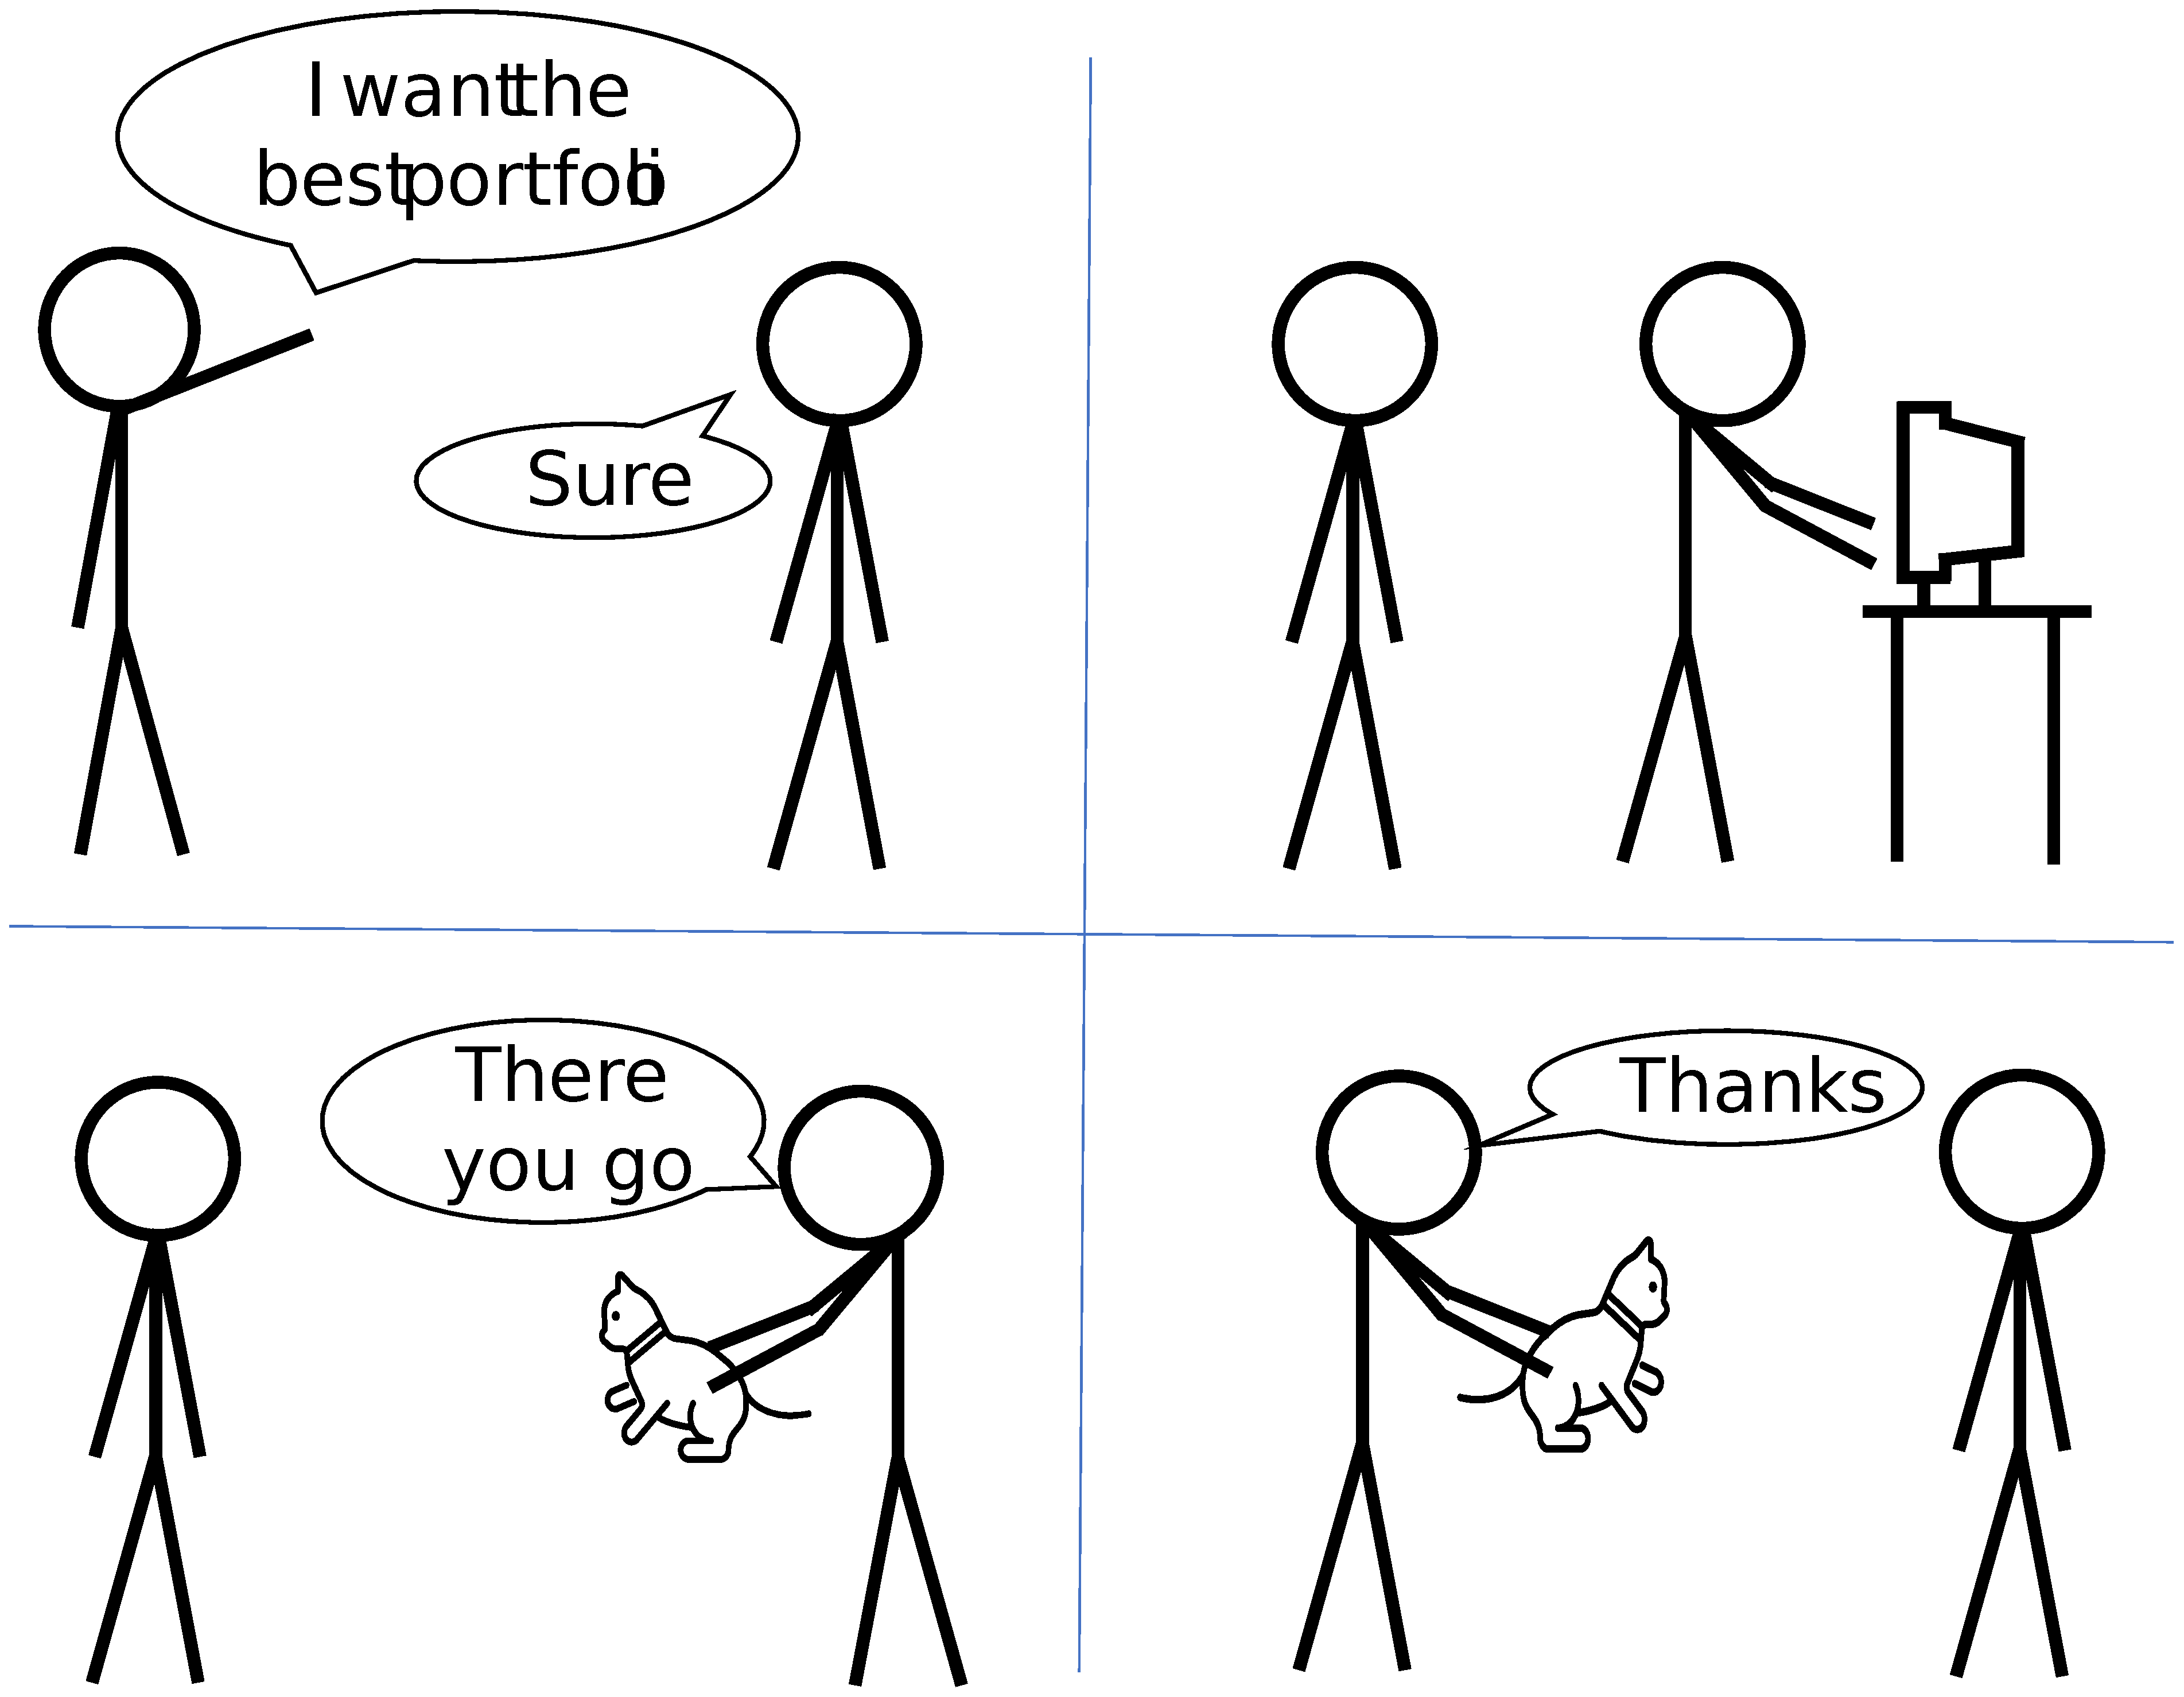
\includegraphics[width=1\textwidth]{imgs/ch2/what_is_a_portfolio.eps}
    \includesvg[width=1\textwidth]{imgs/ch2/what_is_a_portfolio.svg}
    \caption[Portfolio optimization]{Portfolio optimization}
    \label{fig::what_is_a_portfolio}
\end{figure}


\subsubsection{Portfolio Theories} \label{sec::2_portfolio_theories}
At its core portfolio theories attempt to describe the internal structure of a collection of assets that are given the name of portfolio, each asset have a set of attributes (price, liquidity) which can change over time and attributes of the portfolio can be derived as a combination of the attributes of the assets that conform it. Some theories try to separate themselves from pricing mechanisms or more broadly from the specific methods used for the determination of the assets attributes. Below the most relevant portfolio theories to this project are presented in chronological order pointing out the major contributions/features with respect to their predecessors.

\textbf{Classical Portfolio Theory, 1952:} This theory is built around ``probability beliefs", meaning beliefs of people have around how assets will behave in the future expressed in probabilistic terms, and although being widely referenced as a portfolio theory it does not explicitly states what a portfolio is but how to select a portfolio. Introducing a boundary of efficient portfolios with extreme returns and variance of returns combinations. Moreover during the optimization process it assumes that each asset has a known market price distribution over time whose parameters are obtained beforehand, but it does not address how such values should be obtained and leaves it as an assumption of the model \cite{classical_portfolio_theory}.

\textbf{Modern Portfolio Theory of Dynamic Asset Pricing, 1992:} This theory when taken in a discrete setting introduces the representation of a portfolio $\theta$ as an array of securities. In this theory the uncertainty over a time period is modelled via the dividend matrix $D \in \R^{N\times S}$ representing for N securities and S states those securities can be in (only one of the states will be true), each entry $D_{ij}$ represents ``the units of accounts paid by the security i on state j".  Among some concepts introduced are the security price $q=D\psi  \in \R^N$ were $\psi$ is the state-price vector interpreted as ``the marginal cost of obtaining an additional unit of account in state j" \cite{DAP}. 

\textbf{\ac{BPT} \& Mental accounting, 2000:} \ac{BPT} models a Portfolio as a set of portfolios each with its own objectives and performance and computes optimal portfolios as an aggregatios of subportfolios. The mental accounting framework  provides structure to this type of portfolio and a definition of risk to it as the probability of failing to reach the threshold level of return in each mental account \cite{behaviouralPortfolioTheory2000, mental_accounting_10}. 

\textbf{\ac{SPT}, 1995:} \ac{SPT} models the portfolio $\pi(\cdot)$ as a series of stochastic processes each representing the amount invested in a stock at a given time, the value of each asset is calculated by multiplying the amount invested with a wealth process $V^{\pi,w}$, a stochastic process that can depend on the portfolio and initial capital ``$w$" \cite{stochastic_portfolio_theory_2009}. 

\textbf{Model-free Portfolio Theory, 2023:} This model removes the assumption of an underlying probabilistic models for the assets in the portfolios, instead it proposes that each asset has a deterministic price trajectory and proposes the formulation of functionally generated portfolios \cite{model_free_portfolio_theory}. Moreover its derivation is based from a combination of \ac{SPT} with the theory of rough paths which is used to model the internal state of a system (like asset price) with an external control without having to guess a precise nature of the governing differential equations \cite{rough_paths_02} . 

\subsubsection{AirBorne portfolio modelling}
With the exception of \ac{BPT} all portfolios are modelled as a link between an identifier for an asset and a mathematical object, and \ac{BPT} can be identified as a sequence of sub-portfolios with the same structure.

The hashmap structure in Julia is known as a dictionary and an instance of it can be created following Listing \ref{lst:portfolioExample}.

\begin{lstlisting}[language=Julia,escapeinside={(*}{*)},label={lst:portfolioExample},caption={Example of portfolio model instantiation in Julia},captionpos=b]
portfolio_instance = Dict()
\end{lstlisting}

\subsection{Assets and Asset Pricing}
\subsubsection{Assets}
Assets are financial instruments that can be bought or sold, they have two fundamental characteristics, its \textbf{current price} also known as the asset state 
price and its \textbf{future payments} \cite{assetPricing}.

\textbf{Future payments:} In equity stocks may pay dividends that are uncertain and depend on the performance of the company. Other assets may be bonds which deliver predetermined coupon payments which are issued by countries or corporations with the risk of the issuer defaulting. Similar future payments be established for derivatives. A \textbf{dividend} is defined as the payment of an asset at any given time \cite{assetPricing}. 

Given the uncertainty of future payments stochastic processes can be used as a modelling tool for them\cite{assetPricing}.  

\subsubsection{Asset Pricing}
Asset pricing provides a framework to the relationship between returns and risks,  through a hypothesized behaviour of investors, hypothesizing the expected returns through an ``Asset Pricing Model" \cite{investment_management_book_2010}. 

Asset pricing models can be categorized into ``positive" and ``nominative" models, the first simply hypothesise what the price is, whilst the latter hint what it should be \cite{investment_management_book_2010}. 

Some models such as Capital Asset Pricing models, solely attempt to predict the a measure/estimate of the return expectation over risk , modelled  as an intrinsic variance/noise of the return value \cite{investment_management_book_2010}. But is not suitable to calculate variations of asset state-prices over time \cite{assetPricing}. 

\subsubsection{Returns}   \label{sec::ch2_returnDef}
The return is defined as a gain from holding an asset over a period of time. Using this definition two types of returns can be distinguished; \textbf{nominal returns} which are returns expressed in terms of units of a certain currency and \textbf{real returns} which are gains in terms of purchasing power \cite{assetPricing}.

\subsubsection{AirBorne Asset Modelling}
AirBorne models an asset as a quantity held a certain ``assetId", this can be related to an entry in a hashmap. 

The returns of holding an asset over time is calculated by an through the Asset Valuation submodule in the data processing layer of the software introduced in Section \ref{sec::ch4_AssetValuation}, in this same module the overall return of a portfolio is also defined following the same definition of Section \ref{sec::ch2_returnDef}, this allows for many market models, engines and strategies to share the same valuation methods and be comparable to each other.

The state-price on the other hand is defined during the execution of the order by a Market Model, which is addressed in Section \ref{sec::ch4_MarketModelling}, this is because the price paid for an asset can fluctuate based on Market Impact models introduced in Section \ref{sec::market_impact}.


\subsection{The investment management process}
Following the work of Fabozzi the process of investment management can be split into five tasks \cite{investment_management_book_2010}. 
\begin{enumerate}
    \item Setting investment objectives %TODO: define
    \item Selection of investment policy %TODO: define 
    \item Selection of investment strategy %TODO: define
    \item Portfolio construction %TODO: define
    \item Measurement of investment performance %TODO: define
\end{enumerate}

\textbf{Portfolio strategy:} The strategy selects the specific assets to be included in the portfolio. There are two classifications for portfolio strategies; \textit{active} which uses available information and forecasting techniques to achieve a better performance than a broadly diversified portfolio and \textit{passive} which takes a \textbf{minimal expectation input} and \textbf{diversification} to match performance of an \textbf{index} assuming all information is contained in the market price \cite{investment_management_book_2010}.

\textbf{Portfolio construction:} During the construction an investor strives to build an \textit{efficient portfolio}, i.e., one that provides the greatest expected return (given some risk) or lowest risk given a return. Here risk needs to be quantified and three inputs are often needed, \textbf{future expected return}, \textbf{variance of asset return}, \textbf{correlation of asset return} \cite{investment_management_book_2010}.

\textbf{Measurement of investment performance:} Is the calculation of the return realized by a portfolio manager over some time interval, the \textit{``evaluation period"} \cite{investment_management_book_2010}. Is worth pointing out the distinction between the portfolio and the portfolio manager at this point as the portfolio manager is the one making decisions affecting the composition of the portfolio. There are three aims to performance evaluation first if the portfolio manager outperforms a pre-established benchmark, second identification on how the calculated return was achieved and lastly assessing if the the performance was achieved by skill or luck \cite{investment_management_book_2010}.

There are 2 approaches to for the measurement of investment performance by a portfolio manager; \textbf{single-index performance} and \textbf{performance attribution} which decompose the portfolio return so that a client how a portfolio manager achieved its return \cite{investment_management_book_2010}. 

\textbf{Considerations on profit:} Tax factors should be included when considering an investment policy \cite{investment_management_book_2010}.

\subsubsection{Measures}
\textbf{Sharpe ratio:} Originally introduced for portfolio selection, the usage of Sharpe ratio can only be used if there are three elements defined first a notion of a risk free return, and two estimations around the behaviour of the portfolio in the future \textbf{Expected return} and \textbf{Standard deviation of expected returns}. It is assumed that any portfolio expected return can be modelled linearly against a deviation from the risk free rate and thus one maximizing the sharpe ratio (\ref{eq::def_sharpe}) would be optimal \cite{sharpe_ratio_og}.
\begin{equation}
    \label{eq::def_sharpe}
    SR = \frac{\text{Expected return} - \text{Risk free return}}{\text{Standard deviation of expected returns}}
\end{equation}

\textbf{Dollar return:} The advantage of the dollar return (\ref{eq::dollar_return})is that one does not need to have a probabilistic model of the return, however one must be able to measure the market value of a portfolio at particular time instants to be able to calculate it \cite{investment_management_book_2010}.
\begin{equation}
    \label{eq::dollar_return}
    R_p = \frac{MV_1 - MV_0 + D}{MV_0}
\end{equation}
\begin{enumerate}
    \item $R_p = $ Portfolio's return
    \item $MV_1 = $ Portfolio's market value at end of evaluation period.
    \item $MV_0 = $ Portfolio's market value at start of evaluation period.
    \item $D = $ Cash distributions from the portfolio to the client during the evaluation period.
\end{enumerate}

\textbf{Single Period Portfolio Return:} The return of a portfolio of assets over a single period (\ref{eq::single_period_portfolio_return}) can be calculated as the weighted sum of the return of the individual assets in the portfolio. It can also be referred as holding period return or ex post return \cite{investment_management_book_2010}.

\begin{equation}
    \label{eq::single_period_portfolio_return}
    R_p = w_1R_1+w_2R_2+\mathellipsis+w_GR_G
\end{equation}
\begin{enumerate}
    \item $R_p = $ Portfolio's return over the period
    \item $R_g = $ Return of asset g over the period market value at end of evaluation period.
    \item $w_g = $ Weight of asset g in the portfolio (i.e., market value of asset g as a proportion of the market value of the total portfolio)
\end{enumerate}

\textbf{Single Period Portfolio Expected Return:} Similarly the expected return of a portfolio over a single period (\ref{eq::single_period_portfolio_expected_return}) can be defined when returns are modelled through a probability distribution, usually the probability distribution is fitted from  historical data under the assumption that no significant changes should arise during the evaluation period \cite{investment_management_book_2010}.

\begin{equation}
    \label{eq::single_period_portfolio_expected_return}
    E(R_p) = w_1E(R_1)+w_2E(R_2)+\mathellipsis+w_GE(R_G)
\end{equation}

% TODO: Decide if I may include it or not. (Probably won't add VaR to AirBorne)
% \textbf{\ac{VaR}}: \ac{VaR} provides a measure of the amount of capital that can be loss due to unexpected changes in the price or rates of traded instruments in the market \cite{VaR97}. 


\subsubsection{Constraints}

\begin{enumerate}
    \item \textbf{Client-imposed constraints:} Set by the fund manager like concentration limits, restriction on securities types \cite{investment_management_book_2010}.
    \item \textbf{Regulatory constraints:} Concentration limits, restriction on securities types \cite{investment_management_book_2010}.
\end{enumerate}



\subsubsection{AirBorne investment management implementation}
In AirBorne the investment manager is what we call a strategy, a function that given a state (a combination of past and present data) produces a set of orders to be executed by a market given a simulation engine.

The performance evaluation

\subsection{Portfolio Selection}

Portfolio selection is the process of forming a portfolio that optimizes expected returns given an acceptable level of risk, it provides the methods to obtain optimal portfolios and is in general independent of the pricing model used for individual assets \cite{investment_management_book_2010}. 

Diverse and novel approaches for portfolio selection has been put forward in recent years.

\begin{enumerate}
    \item \textbf{\ac{RO}:} \ac{RO} is used as a general tool for optimization under uncertainty, this allows the incorporation of errors around nominal estimates of models such as mean-variance model \cite{robust_optimization_portfolio_selection_21}. 
    \item \textbf{\ac{EA}s:} A niche application of evolutionary algorithms present the \ac{DETS} for forex and equity portfolio optimization \cite{evolutionary_algorithm_22}.
    \item \textbf{\ac{MPC}:} \ac{MPC} is used as a form of adaptive control by leveraging predictions of attributes around assets and using variables such as the ratio portfolio invested on each asset to minimize a cost functional that leads to an optimal portfolio over a period of time, given the accuracy of the predictions \cite{MultiPeriod_PO_mpc}.
\end{enumerate}


\subsubsection{Mean-Variance portfolio analysis}
Mean-Variance Portfolio Analysis is a normative theory for portfolio selection, meaning that aims to describe the behaviour investors should follow to form an optimal portfolio \cite{investment_management_book_2010}.

A well known portfolio selection technique is the Marowitz strategy, in this technique the returns over a number of assets is modelled as a multidimensional random variable, (i.e., a multivariate gaussian), afterwards one gathers a sample of returns over a certain time window, and estimates the expected return vector and correlation matrix of the sample. Then it is assumed that in the near future the behaviour of the returns should follow the same distribution and the objective of the problem is given a certain overall expected return desired to obtain the distribution of assets that minimizes the total variance \cite{classical_portfolio_theory}.

In this project a state of the art \ac{MPC} controller will be tested following a Mean-Variance framework (described in Section \ref{ch3}), where given predictions on the return and the variance of the portfolio a linear quadratic form, quadratic on the variance and linear on the expected return is minimized over a series of time \cite{MultiPeriod_PO_mpc}.

\subsubsection{Airborne portfolio selection implementation}
A simple portfolio selection strategy using the Markowitz strategy can be implemented in Julia following Listing \ref{lst:markowitzExample}, AirBorne provides out of the box a strategy that implements the Markowitz strategy following a very similar code.

\clearpage

\begin{lstlisting}[language=Julia,escapeinside={(*}{*)},label={lst:markowitzExample},caption={Markowitz example in Julia using Direct Search},captionpos=b]
# Let returnHistory be a DataFrame with one column per assetId
# and one row per sampled time.
using DataFrames
using DirectSearch
horizon=10
min_growth=0.001 # Minimum desired growth in one interval
d = returnHistory[(end - horizon + 1):end, :] # History of returns
M = covariance(d) # Covariance Matrix
m = mean(Matrix(d[!, :]); dims=1)
max_return, ix = findmax(m)

if max_return > min_growth # Feasible problem
    initial_point = zeros(size(m)) # Warm start solution
    initial_point[ix] = 1.0

    upper_cons(x) = all(x .<= 1)
    lower_cons(x) = all(x .>= 0)
    min_return(x) = min_growth - (m * x)[1] # I want at least a 0.1% return in 1 day 
    obj(x) = x' * M * x

    p = DSProblem(length(m))
    SetGranularity(p, Dict([i => 0.001 for i in 1:length(m)]))
    SetObjective(p, obj)
    AddProgressiveConstraint(p, min_return)
    AddExtremeConstraint(p, upper_cons)
    AddExtremeConstraint(p, lower_cons)
    SetInitialPoint(p, vec([i for i in initial_point]))
    Optimize!(p)
    solution = isnothing(p.x) ? zeros(size(m)) : p.x
else
    solution = zeros(size(m)) # Sell absolutely everytihng. Market is going down.
end

\end{lstlisting}

\subsection{Optimal Execution or Portfolio Liquidation}
A separate (although not always needed if already accounted in the portfolio selection step) is known as \textbf{Optimal Execution}, usually happens once a particular portfolio or change in portfolio composition is selected, this means that the final portfolio composition at a certain time is known (as well as the initial composition of the portfolio) \cite{OptimalExecutionReview}.

The objective is to minimize the costs from moving from one portfolio configuration to another \cite{OptimalExecutionReview}. A simple application is of brokers collecting orders from multiple portfolio managers and combining them into a metaorder \cite{slides_on_optimal_execution}.  

\begin{quote}
    Metaorder: ``An execution performed by a single Broker, on a single stock, in a given direction. All metaorders are completed within a trading day \cite{slides_on_optimal_execution}."
\end{quote}

During the execution phase, particularly when large orders are considered it is extremely important to consider the effect of the application of the order on the market price, this known as market impact.

\subsubsection{Market impact} \label{sec::market_impact}
Market impact is the influence of the transaction on the price of equity, it gains relevance as one places orders in the market the price may fluctuate, this combined with the execution cost creates a trade-off between placing large orders or splitting such order into a sequence of smaller orders \cite{FinancialMathematics_marketImpact}. Some of the models used in literature are:

\begin{enumerate}
    \item \textbf{Hausman, 1992:} Used ordered probit to estimate the fluctuation of the price of a selected, very liquid sample of stock in the US during 1988 given their transactions \cite{hausman_marketImpact_probitModel}.
    \item \textbf{Bertsimas and Lo, 1998:} Introduced given a "price-impact" function the optimal execution of large orders using dynamic programming in 1998 \cite{Bertsimas_early_marketImpact}.
    \item \textbf{Almgren and Chriss, 1999:} Similarly Almgren and Chriss split the impact into a transient and permanent component, each can be non-linear in principle although a linear impact is presented as a special case \cite{almgren2001optimal}.
\end{enumerate}


\subsubsection{Airborne optimal execution implementation}

Airborne provides out of the box functions to compute optimal execution, following an affine fee structure with respect to the value of shares purchased under the assumption of a stiff market were the price of each unit of asset does not change with the amount.

Listing \ref{lst:optimalExecutionExample} shows the logic behind an optimal execution solution provided on the \textbf{Static Market} model were one tries to minimize the loss of value on a transaction subject to fixed and variable fees for each transacted asset (\ref{eq::optimalExecutionExample}).



\begin{equation}
\label{eq::optimalExecutionExample}  
\begin{aligned}
& \max_{d} k   \\
\text{s.t.} & k\geq 0 \\
& D1 + d  - \hat{e}_{c} * \left(\alpha_v |d| + \alpha_f \sum{(1-\delta_{\odot}(d))}  \right) = D2 * k
\end{aligned}
\end{equation}

\begin{enumerate}
    \item $D_1$: Initial distribution of value of the portfolio, vector of norm 1 (in dollars).
    \item $D_2$: Final distribution of value of the portfolio, vector of norm 1 (in dollars).
    \item $\hat{e}_{c}$: Vector with 1 on the entry representing the currency fees.
    \item $k$: Value of final portfolio with respect to initial.
    \item $d$: Dollars to buy/sell of each asset (vector).
    \item $\alpha_v$: Proportional cost with respect to transacted amount (scalar quantity)
    \item $\alpha_f$: Fix cost per transaction (scalar quantity)
\end{enumerate}

\begin{lstlisting}[language=Julia,escapeinside={(*}{*)},label={lst:optimalExecutionExample},caption={Optimal Execution example in Julia using JuMP and Ipopt},captionpos=b]
using AirBorne.Utils: (* \delta{} *)
using JuMP: Model, @variable, @objective, @constraint, optimize!, value, set_silent
using SparseArrays: sparse, I, spdiagm, SparseVector
using Ipopt: Ipopt
import MathOptInterface as MOI
# Generate Source Distribution from Portfolio
D1 = sourceDst; D2 = targetDst
curency_symbol = "FEX/USD";
curency_pos = findall(x -> x == curency_symbol, [x for x in keys(D1)])[1]
e_c = SparseVector(N, [curency_pos], [1]) # Dollar Fees Vector
N = length(sourceDst)
M = zeros(N, N)
M[curency_pos, :] = propShareVal .* -1 # Price to pay per share (without fees)
P = spdiagm(0 => propShareVal) + M
##### Optimization Problem
genOrderModel = Model(Ipopt.Optimizer)
@variable(genOrderModel, 0 <= k) # Proportionality factor (shrinkage of portfolio)
@variable(genOrderModel, d[1:N])  # Amount to buy/sell of each asset
@variable(genOrderModel, fee_v >= 0) # Amount Proportional Fees
@constraint(genOrderModel,[fee_v; d.* (*\alpha*)_v] in MOI.NormOneCone(1 + N)) # Norm-1
@variable(genOrderModel, fee_c >= 0) # Number of transactions fees
@constraint(genOrderModel, fee_c == sum(-(* \delta{} *).(d) .+ 1) * (*\alpha*)_f) 
@constraint(genOrderModel, d[curency_pos] == 0) # Do not buy or sell dollars (this is the currency).
@constraint(genOrderModel,D1.+P*d.-(e_c.*(fee_v + fee_c)).== D2.* k) # D1+ P*d-Fees->D2*k
@objective(genOrderModel, Max, k) # With variance minimization
optimize!(genOrderModel)
d = value.(d)
\end{lstlisting}
\chapter{Optimal Control}
\label{ch3}

%%%%%%%%%%%%%%%%%%%%%%%%%%%%%%%%%%%%%%%
% IMPORTANT
\singlespacing % THESE THREE
\minitoc % LINES MUST APPEAR IN
\doublespacing % EVERY CHAPTER
% COPY THEM IN ANY NEW CHAPTER
%%%%%%%%%%%%%%%%%%%%%%%%%%%%%%%%%%%%%%%

\section{Mean-Variance MPC Framework}

\subsection{Introduction to MPC}

\ac{MPC} is a control technique in which given a state space $X$ and control variables on the input space $U$ over a certain time horizon $T$, the control law selected is such that the objective function (that depends on the state and input values) is minimized/maximized subject to constraints over the horizon \cite{PredictiveControl}. After the control law is selected a certain number of control sequences are applied before repeating the procedure.

Moreover several optional modifications can be done to the controller to make it more adaptive to disturbances or  mismatches against the physical system, as well as to improve its computational efficiency over time by introducing  model parameter estimation or variable horizon functionalities in the loop, this can be done either before the optimization routine begins during "Pre-checks" or afterwards during "Post-checks", for example after the optimization routine ends if there are any constraint violations one could increase the sampling frequency, or given the current state one could decide to reduce the horizon. 

Figure \ref{fig::ch3_MPC} shows a diagram representing the MPC overall algorithm.

\begin{figure}[h!]
    \centering
    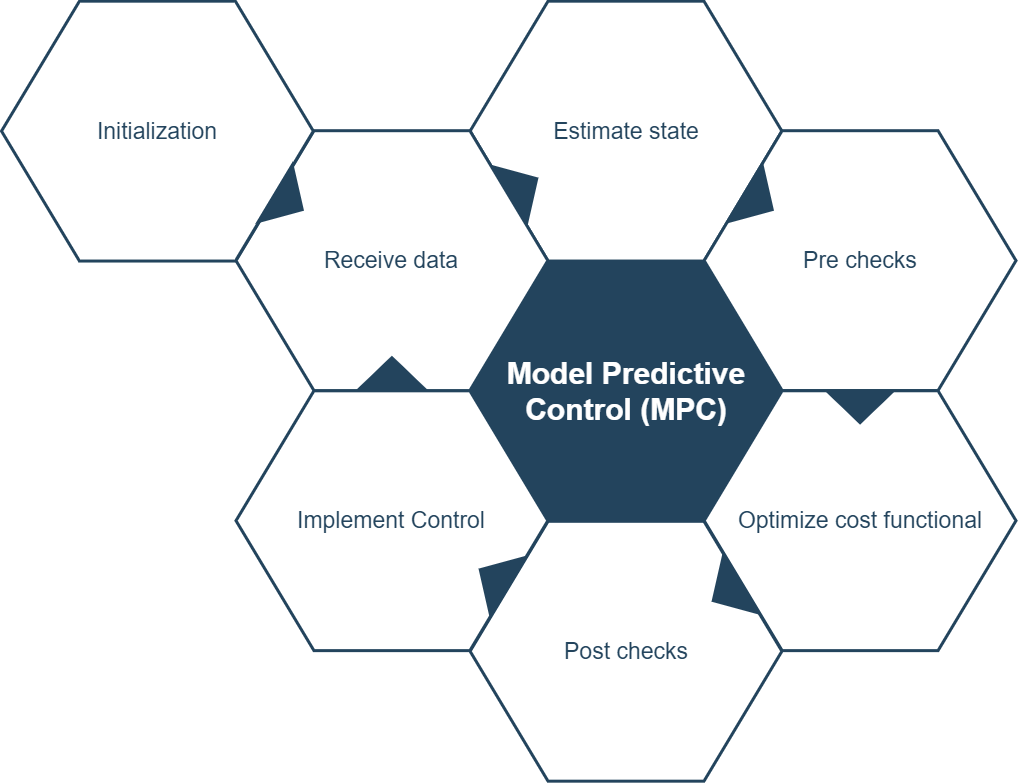
\includegraphics[width=1\textwidth]{imgs/ch3/MPC drawing.png}
    \caption[\ac{MPC} logic diagram]{\ac{MPC} logic diagram}
    \label{fig::ch3_MPC}
\end{figure}

In this section the elements of the model predictive control used in this project are introduced. With particular emphasis to its application in multi-period portfolio optimization. Many of elements of this formulation can be attributed to the paper published by Xiaoyue Li in 2022 \cite{MultiPeriod_PO_mpc}.

\subsection{Formulation}
This method tries to solve a \ac{LQP}  were the cost functional has a negative quadratic term for each daily(transition) variance day and a positive linear term for returns \cite{MultiPeriod_PO_mpc}. By minimizing such cost functional a trade-off between expected risk (variance) and expected returns is achieved, not in a ratio sense like optimizing Sharpe but in opposing forces of a \ac{LQP}  problem \cite{MultiPeriod_PO_mpc}. 

Letting $N$ be the number of assets considered for the optimization problem.

\textbf{State Space:} The vector of expected returns and the covariance matrix at each point in time, $\left[r_{t+1|t},...,r_{t+H|t}\right]$ and $\left[\Sigma_{t+1},...,\Sigma_{t+H}\right]$, where $r_i \in \R^N$ and $\Sigma_i \in \R^{N\times N}$, therefore the state space {T()}belong in $\R^{H \times N\times(N+1)}$.

\textbf{Input Space:} The control variable in this formulation is the allocation of assets with respect of the total value of the portfolio at each point in time, represented by $\left[\pi_{t+1},...,\pi_{t+H}\right]$.

\textbf{Objective Function:} A quadratic form (\ref{eq::c3_Objective}) to maximize the expected return given a quadratic cost in term of the uncertainty with a proportional cost on the transacted ratio.

\begin{equation} \label{eq::c3_Objective}
\max_{\pi_{t+1},...,\pi_{t+H}} \left(\sum_{\tau=t+1}^{\tau=t+H} \hat{r}^{T}_{\tau|t}\pi_{\tau} 
- \gamma^{risk}\left(\pi_{\tau}^T \hat{\Sigma}_{\tau|t}\pi_{\tau}\right) 
- \gamma^{trade}||\pi_{\tau}-\pi_{\tau-1}||_1
\right)
\end{equation}
The hyper-parameters of the objective function are $\gamma^{risk}$ the tisk aversion parameter and $\gamma^{trade}$ the transaction cost.


\textbf{Constraints:} The basic constraints in this problem are that all entries in allocation vector to be greater or equal than zero, which is equivalent to no edging (\ref{eq::ch3_noEdgingConstraint}), and that the sum of the allocation at any point in time adds up to 1 (\ref{eq::ch3_unitAllocationConstraint}).

\begin{equation}\label{eq::ch3_noEdgingConstraint}
\pi_{\tau}\geq 0\quad \forall\tau=t+1,...,t+H
\end{equation}

\begin{equation}\label{eq::ch3_unitAllocationConstraint}
\textbf{1}^T\pi_{\tau}=1 \quad \forall\tau=t+1,...,t+H
\end{equation}

Also it is possible to place constraints on the returns at any point in time (\ref{eq::ch3_iReturnConstraint}), or forbid holding shaeres of a particular company ``$j$" assets at time $\tau$ (\ref{eq::ch3_forbidAssrtConstraint}).

\begin{equation}\label{eq::ch3_iReturnConstraint}
 \hat{r}^{T}_{\tau|t} \pi_{\tau} - \text{minVal} \geq 0
\end{equation}

\begin{equation}\label{eq::ch3_forbidAssrtConstraint}
  \pi_{\tau,j} = 0 
\end{equation}


Or by assuming the returns distribution in each time to be independent from each other, one can use the overall expected return between time $t$ and $i$ at $t$ (\ref{eq::ch3_overallReturn}) to define more complex constraints such as ``minimal accumulated expected return at time i" (\ref{eq::ch3_iAccumReturnConstraint})
``Minimum portfolio value"(\ref{eq::ch3_iMinPortfolioConstraint}).


\begin{equation}\label{eq::ch3_overallReturn}
    \hat{r}_{[t,i|t]}=\prod_{\tau=t+1}^{i} \hat{r}^{T}_{\tau|t}\pi_{\tau} - \gamma^{trade}||\pi_{\tau}-\pi_{\tau-1}||_1 
\end{equation}

\begin{equation}\label{eq::ch3_iAccumReturnConstraint}
    \hat{r}_{[t,i|t]} - \text{minVal} \geq 0
\end{equation}


\begin{equation}\label{eq::ch3_iMinPortfolioConstraint}
   \text{initialCapital} \hat{r}_{[t,i|t]} - \text{minPortfolioVal} \geq 0
\end{equation}

Finally constraints such as initial capital amount, are implemented as parameters of the MPC whilst the control variable operates on portfolio scaled by the initial capital. 

\textbf{System dynamics:}
In order to estimate the dollar value of the composition of the portfolio over future periods of time it is necessary to be able to estimate the value of different assets over time or more precisely the expected period return. This is done through forecasting.

\subsection{Forecasting}

In this section the forecasting/estimation of the return vector and covariance matrices is addressed, first a brief discussion on causality between measurable attribute and asset prices will be carried out, followed by descriptions of several forecasting methods used in the experiments on Chapter \ref{ch5}.

It is important to notice that a necessary condition for the objective function (\ref{eq::c3_Objective}) to output sensible input sequences when optimized is for the covariance matrices to be positive definite. Some of the methods do not guarantee such result, for those methods the objective function (\ref{eq::c3_Objective}) is modified to not include the quadratic terms.

\subsubsection{Discussions on causality}
Before proceeding into the specifics of the model is worth studying the potential causality between attributes of assets, either causal relationship between assets, that can come in different shapes. Since the nature of the model in the model-free formulation won't be guessed the factors to be taken into account for the model should have some degree of relationship between each other in order to make more useful control systems, meaning to have a model capable of better predictions when considering the effect of controllable variables and other state variables.

\begin{enumerate}
    \item Do poor performance of agricultural companies have a domino effect on the performance of other companies in the Food industry or fashion industry and can this be observed through the stock price?
    \item Can changes in the price and traded volume may affect each other, therefore can there be a bi-directional causality may exist as in a closed loop system?
    \item Can broad macro-economic factors influence the overall direction of stock prices?
    \item Can regulatory reforms impact the dynamics between attributes with causal relationships?
    \begin{enumerate}
        \item What about market structures such like monopolies and cartels? 
        \item Under what conditions can we assume causal relationships can be maintained? 
        \item How fast the algorithms need to be in order to adapt to unobservable events as regulatory or market power changes, meaning how long into the past a human observer need to be aware of changes that can affect the thrust-worthiness of the output of the model?
    \end{enumerate}
\end{enumerate}   

\textbf{Price-Volume causality:} Price volume causality is a widely studied subject with mixed results and no clear general answer, from an abstract point of view for each sale that happens there must have been a purchase, therefore the amount of sales and its price don't need to be related however at closer inspection under particular circumstances there may be evidence of the contrary. 

There are individual pieces of evidence that suggest a causal relationship between price and volume as in the case of the GameStop frenzy were the timing of the selling and buying of shares of GameStop forced the price to go up and forced many short-sellers to liquidate their positions in a distressed sale \cite{game_stop_case}. Although this example is a form of predatory trading that carries with it a deep ethical discussion it does show that is possible to affect price with volume and likely vice versa, at least under particular circumstances.

A study in the stock exchange in India suggest by using Granger causality suggest that the causality between volume traded and price fluctuate over time depending on market reforms and presence of feedback trading between 95'and 21' having price driving volume and after 21' no relation \cite{price_volume_causality_india06}.

A more recent study suggest that the Granger test for linear causality and its extension by Hiemstra and Jones for nonlinear Granger causality is prone to over-rejection by using Monte Carlo simulations and introduced a model free test based on conditional permutation-entropy to measure nonlinear causality. This method was applied to the SP500 between 1950 and 1990 and it suggested the existence of a causal relationship between price and volume both on mean and variance for daily trade \cite{price_volume_causality_enthropy}.

\subsubsection{Behavioural forecasting}
This method is a modified version of the \ac{DeePC}\cite{og_deepc}, which is arises from an application of the fundamental lemma of behavioural systems \cite{precursor_deepc,fundamentalLemma}. Is worth noticing that in its application one of the hypothesis has been relaxed in particular the one of the controllability of the system.

The fundamental lemma states that for a \ac{LTI} controllable system any trajectory in the input-output space can be expressed as a linear combination of past trajectories \cite{fundamentalLemma}. Lets consider the Hankel matrix (\ref{eq::hankelMatrix}) of an autonomous system with output $y$ which at time t takes the value $y_t$, this matrix on each column contains trajectories of length $N$. 

\begin{equation}
    \label{eq::hankelMatrix}
    H(y)= \begin{bmatrix}
y_1 & \cdots & y_{t-N+1}\\
\vdots & \ddots & \vdots\\
y_N & \cdots & y_t
\end{bmatrix}
\end{equation}

Now consider two integers $p$ and $f$ such that $p+f=N$ and $p\geq1$, $f\geq1$, termed past and future windows. Lets also split the Hankel matrix into the past and future Hankel submatrices (\ref{eq::hankelMatrixpf}). Furthermore, consider that we have knowledge of the past $p$ values of the output $y$, the trajectory of the past $p$ values can be determined as a linear combination of the columns of $H_p(y)$ such that $g=H_p(y)\backslash  y_{t-p+1:t}$. the behavioural forecasting predicts the following $f$ values of $y$ as the linear combination of $\hat{y}_{t+1:t+f} = H_f(y)*g$ 

\begin{equation}
    \label{eq::hankelMatrixpf}
    H(y)= \begin{bmatrix}
y_1 & \cdots & y_{t-N+1}\\
\vdots & \ddots & \vdots\\
y_p & \cdots & y_{t-p+1} \\
y_{p+1} & \cdots & y_{t-p+2} \\
\vdots & \ddots & \vdots\\
y_N & \cdots & y_t
\end{bmatrix}\Rightarrow{} \quad 
\begin{array}{l}
H_p(y)= \begin{bmatrix}
y_1 & \cdots & y_{t-N+1}\\
\vdots & \ddots & \vdots\\
y_p & \cdots & y_{t-p+1} 
\end{bmatrix}\\
 H_f(y)= \begin{bmatrix}
y_{p+1} & \cdots & y_{t-p+2} \\
\vdots & \ddots & \vdots\\
y_N & \cdots & y_t
\end{bmatrix}
\end{array}
\end{equation}

\subsubsection{Hidden Markov Model (\ac{HMM})}

\ac{HMM} is a method that predicts the expected return vector and the covariance matrix to be in a discrete set of states that are not directly observable, each state is represented as a time-invariant stochastic process were at each time-instant the returns follow a  Multivariate Gaussian distribution with fix mean vector and covariance matrix \cite{MultiPeriod_PO_mpc}.

Given past data, the Baum-Welch method \cite{OG_BaumWelch} is used to estimate the transition probability between these hidden states and the coefficients of the MultiVariate Gaussians associated to each hidden state.

Using recent past data the current state is estimated, and the forecast of covariance and mean vectors is computed in an iterative manner, is worth pointing out that at the moment the ``HiddenMarkovModels.jl" package \cite{HiddenMarkovModels.jl} in Julia just estimates the most likely state, and it doesn't provide the most likely probability distribution of states, which could be used for a refinement of the forecast vectors and matrices.

A huge advantage of this method is that if the coefficients of the HMM are not modified significantly the forecast matrices will only depend on the current state, and it can be precomputed and save in memory.

Following the work of Guidolin \cite{numberOfRegimes} two states known as ``bull" and ``bear" (or ``normal" and ``contraction") shall be used in the \ac{HMM}, . Thus the transition matrix between the states (\ref{eq::ch3_HMM_TransitionMatrix}) is a $2\times2$ matrix where $p_{nn}$ is the probability of remaining in the normal regime, whilst $p_{cc}$ is the probability of remaining on the contraction regime following the notation of Li \cite{MultiPeriod_PO_mpc}.

\begin{equation} \label{eq::ch3_HMM_TransitionMatrix}
    T_{hmm}=\begin{bmatrix}
        p_{nn} & 1- p_{nn} \\
        1-p_{nn} & p_{cc} \\
    \end{bmatrix}
\end{equation}

During the normal regime the model assumes the returns to follow a distribution $\D_n=\Normal{n}$ and during the contraction regime $\D_c=\Normal{c}$. 

\textbf{Forecast algorithm:} Let $q_t=[q_{t,n},q_{t,c}]$ be the probability distribution of the state at time t the forecast algorithm follows Algorithm \ref{algo::HMMForecast} which can be implemented in Julia by adapting Listing \ref{lst:HMMForecast}.

\begin{algorithm} \label{algo::HMMForecast}
    \caption{\ac{HMM} Forecast}
  \begin{algorithmic}[1]
  \Require Determine $q_0,\quad \Normal{n},\quad\Normal{c}$
  \State $V_\mu = \begin{bmatrix} \mu_n \\ \mu_c\end{bmatrix}$   
  \State $V_\Sigma = \begin{bmatrix} \Sigma_n \\ \Sigma_c\end{bmatrix}$   
  \State $\mu_0 = q_0'*V_\mu$
  \State $\Sigma_0 = q_0'*V_\Sigma$ 
    \For{\texttt{i=0:Horizon-1}}
        \State $q_{i+1} = T_{hmm}*q_i$ 
        \State $\mu_{i+1} = q_{i+1}*V_\mu$
        \State $\Sigma_{i+1} = q_{i+1}*(V_\mu + \begin{bmatrix}
           (\mu_n-\mu_{i+1})*((\mu_n-\mu_{i+1})') \\
           (\mu_c-\mu_{i+1})*((\mu_c-\mu_{i+1})')
        \end{bmatrix}$
    \EndFor
  \end{algorithmic}
\end{algorithm}


\begin{lstlisting}[language=Julia,escapeinside={(*}{*)},label={lst:HMMForecast},caption={Example implementation of HMM Forecast in Julia},captionpos=b]
# The following is a Pseudo-code, not intended to be executed alone
    using HiddenMarkovModels
    hmm=...; # Hidden Markov Model variable
    N=length(hmm); # Number of states
    fitDists=[obs_distribution(hmm,i) for i=1:length(hmm)]; # Distributions of each state
    (*V\mu*)= [f.(*\mu*) for f=fitDists]
    (*V\Sigma*)=[f.(*\Sigma*) for f=fitDists]
    q0 = zeros(N);
    q0[get_current_state(hmm,context.extra.obs_seq)] = 1 # Probability of each state at t=0
    (*\mu*)0 = sum(q0.*(*V\mu*)); (*\Sigma*)0 = sum([ q0[i].*(*V\Sigma*)[i] for i=1:N])
    M=length((*\mu*)0) 
    # Pre-allocation of output
    forecast = [(zeros(M),zeros(M,M)) for i=1:futureHorizon] 
    for i=1:futureHorizon
        q1 = transition_matrix(hmm)*q0
        (*\mu*)1 = sum(q1.*(*V\mu*))
        (*\Sigma*)1 = sum([ q1[i].*((*V\Sigma*)[i] + (((*V\mu*)[i]-(*\mu*)1)*((*V\mu*)[i]-(*\mu*)1)'))  for i=1:N]) 
        q0,(*\mu*)0,(*\Sigma*)0=q1,(*\mu*)1,(*\Sigma*)1
        forecast[i][1][1:M]=(*\mu*)1
        forecast[i][2][1:M,1:M]=(*\Sigma*)1
    end
\end{lstlisting}

\subsubsection{Benchmarks}
In order to benchmark the Behavioural and \ac{HMM} methods two basic but well established forecasting techniques will be used as a comparison.

\textbf{Linear regression:} In this method the expected return of each asset over with sample window ``$w_s$" is adjusted through a linear regression over a sample of length $w_{lr}$, this produces an estimate on the expected return vector. 

Is worth pointing out that the same technique cannot be used for the covariance matrix,at least on a per entry level because the matrix is not guaranteed to be positive semi-definite.

\textbf{Last value:} This is the forecasting technique used by the Markowitz strategy, in this technique the future return matrix and covariance matrix is expected to be the same as in the immediate past data over a sample window of individual asset returns ``$w_s$" which can be different for the estimation of expected returns $w_{s\mu}$ and the covariance matrix $w_{s\Sigma}$. 

\chapter{Julia Implementation}
\label{ch4}

%%%%%%%%%%%%%%%%%%%%%%%%%%%%%%%%%%%%%%%
% IMPORTANT
\singlespacing % THESE THREE
\minitoc % LINES MUST APPEAR IN
\doublespacing % EVERY CHAPTER
% COPY THEM IN ANY NEW CHAPTER
%%%%%%%%%%%%%%%%%%%%%%%%%%%%%%%%%%%%%%%


\section{Julia Features}
In this section the most relevant Julia features and limitations for this project are addressed. For each feature relevant links to the official documentation and examples on how they are leveraged in this project are provided.

\subsection{Features}
This section will focus on important features Julia has and the importance of the collection of these features when considering the project at hand.

Some features like multiple dispatch are generally known to be exclusive to the Julia language, however given the shear amount of languages is relatively difficult to claim that no language also has some of them.

Some languages may have workarounds to simulate the features to some extent (i.e. You can create a function in python that re-directs to a function based on the input Types simulating the multiple dispatch behaviour) usually these workarounds require extra computation and thus are not as efficient. The features addressed in this section are natively designed for the Julia language.

\subsubsection{Multiple dispatch}
\cite{julia_performance_tips_multiple_dispatch}

\subsubsection{Metaprogramming}
\url{https://docs.julialang.org/en/v1/manual/metaprogramming/}

\subsubsection{Parametric Types}
\url{https://docs.julialang.org/en/v1/manual/types/#Parametric-Types}

\subsubsection{Output Preallocation}
Julia allows to bypass a common bottleneck, which is memory allocation and garbage collection by preallocating the output of a function \cite{julia_performance_tips}.

In practice this looks like the two excerpts of code below, where the addition of money in potentially different currencies is defined, if the currencies are different we want to form a wallet with both amounts, and if the currencies are the same then we want to have money in the same currency as the ones being aggregated.
\begin{lstlisting}[language=Julia]
# Not Type Stable
Base.:+(a::Money{A}, b::Money{B}) where {A,B} = A==B ? Money{A}(a.value + b.value) : Wallet(Dict(A=>a.value,B=>b.value)) 
\end{lstlisting}
\begin{lstlisting}[language=Julia]
# Type Stable
Base.:+(a::Money{A}, b::Money{A}) where {A} = MoneyH{A}(a.value + b.value) 
Base.:+(a::Money{A}, b::Money{B}) where {A,B} = WalletB(Dict(A=>a.value,B=>b.value)) 
\end{lstlisting}
Looking at the examples is easy to see that the first one is not type stable therefore Julia cannot pre-allocate the output prior to run-time whilst and the second is because two methods are put forward and leveraging multiple dispatch the output type is predictable and memory can be allocated efficiently.

\subsubsection{Module Loading}
Unlike C/C++,  when importing modules (or packages for C) in separate parts of the code the existing module is just made available into the scope instead of being loaded again \cite{julia_differences}. 
\subsection{Constraints and Best Practices}

Language constraints and best practices are not a bad thing per se, constraints are imposed by the structure of the code and is what gives us the guidelines to code itself, without constraints there would be no structure to follow. Best practices are structures that if not violated will improve either computational efficiency, readability or maintainability/future proofing of the code.

\subsubsection{Type stability}
If the type of the output of a function is predictable and does not depend on the specific values of the input the code in julia is faster, this is because the type of the output of the function can be accounted at compilation time \cite{julia_performance_tips, julia_qa_stability}.

\subsubsection{Unicode Input}
A distinguishable feature of Julia is its extended Unicode input this allows to mathematical symbols to be used in the language closing the gap between mathematical modelling and programmatic code representation, albeit unicode representation is not unique to julia, the variety of ``abbreviations" available allow to have expression like the one in the snippet below as part of the code \cite{julia_unicode_input}.

\begin{lstlisting}[language=Julia,escapeinside={(*}{*)}]
(*$\psi$*)=3 
if (*$\psi \in$*) [1,2,3]
    # Do something
else 
    # Do something else
end
\end{lstlisting}

Although it seems like a small gain, it significantly expands the vocabulary available to define variables, and when making code oriented to address needs in field of physics and mathematical allows to align variable names with their counterparts in literature whilst increasing readability by shortening the variable names without losing meaning. Is worth mentioning that other languages such as like Maple and Mathematica also support this feature.



\section{AirBorne Package}
This project delivered the Julia package AirBorne\cite{AirBorne}.

\subsection{High level design}

\subsection{Data layer} 

\subsubsection{Asset Valuation} \label{sec::ch4_AssetValuation}


\subsection{Market Modelling} \label{sec::ch4_MarketModelling}


\subsection{}






% \subsubsection{ARCHModels.jl}
% ARCHModels.jl provides the necessary tools to simulate \ac{ARCH} and \ac{P-ARCH} models \cite{ARCHModels.jl} . 

% The \ac{ARCH} model was originally introduced as a model to simulate inflation on the \ac{UK}, this model is characterized by not having constant variance conditional to the recent past, but overall constant unconditional variance, meaning that recent past provide information about the single period next variance \cite{ARCHModels_og_paper}.  Whereas the \ac{P-ARCH} model was first proposed for modelling the seasonal volatility patter of asset returns were seasonal periodicity on its behaviour can be observed \cite{Periodic_ARCHModels_og_paper} .

% Moreover this package also provides some standard datasets such as: 
% \begin{enumerate}
%     \item ARCHModels.BG96: Data from Bollerslev and Ghysels\cite{Periodic_ARCHModels_og_paper,ARCHModels.jl}.
%     \item ARCHModels.DOW29: Stock returns, in procent, from 03/19/2008 through 04/11/2019, for tickers AAPL, IBM, XOM, KO, MSFT, INTC, MRK, PG, VZ, WBA, V, JNJ, PFE, CSCO, TRV, WMT, MMM, UTX, UNH, NKE, HD, BA, AXP, MCD, CAT, GS, JPM, CVX, DIS \cite{ARCHModels.jl}.
% \end{enumerate}

\subsection{Strategies}
Strategies define the trading logic that an agent implements given data provided by the market.
\subsubsection{\ac{SMA}}
\textbf{Optimization Routine:} 


\chapter{Experimental results}
\label{ch5}

%%%%%%%%%%%%%%%%%%%%%%%%%%%%%%%%%%%%%%%
% IMPORTANT
\singlespacing % THESE THREE
\minitoc % LINES MUST APPEAR IN
\doublespacing % EVERY CHAPTER
% COPY THEM IN ANY NEW CHAPTER
%%%%%%%%%%%%%%%%%%%%%%%%%%%%%%%%%%%%%%%

\section{Data set}


The dataset used in the following experiments is comprised of the top 5 most traded companies in volume according to NASDAQ screener in each sector as per 19\textsuperscript{th} August 2023, listed since 2016 from Jan 1st 2017 until Jan 1\textsuperscript{st} 2022. The resulting companies can be found in Tables \ref{tab:NASDAQ_1} and \ref{tab:NASDAQ_2}  on Appendix \ref{sec::AppendixNasdaqScreener} using the script in Listing \ref{lst:dataGenScript}. The data corresponding to 2017 and 2018 will be used to pre-load the \ac{MPC} with an initial set of data to make predictions with, 2019 will be used as training data, 2020 as validation data and finally 2021 will be used for backtesting.

Both the \href{https://github.com/brunocastroibarburu94/dissertation_msc_2023/blob/main/dissertationFigures/data/cache/Mark1/2023_08_19_16_9_49_915.parq.snappy}{Yahoo Finance ticker data}\footnote{\url{https://github.com/brunocastroibarburu94/dissertation_msc_2023/blob/main/dissertationFigures/data/cache/Mark1/2023_08_19_16_9_49_915.parq.snappy}} and  \href{https://github.com/brunocastroibarburu94/dissertation_msc_2023/blob/main/dissertationFigures/data/cache/NASDAQscreener_Mark1/2023_08_19_17_16_37_731.parq.snappy}{NASDAQ screener data}\footnote{\url{https://github.com/brunocastroibarburu94/dissertation_msc_2023/blob/main/dissertationFigures/data/cache/NASDAQscreener_Mark1/2023_08_19_17_16_37_731.parq.snappy}} is available online on GitHub and are stored in parquet file format whilst compressed with the snappy algorithm.

\clearpage

\begin{lstlisting}[language=Julia,escapeinside={(*}{*)},label={lst:dataGenScript},caption={Data generation script},captionpos=b]
using DataFrames: groupby, combine
bundle_id="Mark1"
cache_dir = joinpath(@__DIR__, "data", "cache")
###    Pick the 5 most traded companies per sector
using AirBorne.ETL.NASDAQ: screener
using AirBorne.Utils: get_latest_N
tickers_df = screener()
filtered_df =tickers_df[[   x!="" ? parse(Int64, x)<2016 : false for x in tickers_df.ipoyear],["symbol","marketCap","sector","volume"]]
filtered_df[!,"volume"]=parse.(Int64,filtered_df[!,"volume"])
filtered_df[!,"marketCap"]=parse.(Float64,filtered_df[!,"marketCap"])
grouped_df = groupby(filtered_df,"sector")
f(sdf)= get_latest_N(sdf,:volume,5;rev=true)
result = combine(grouped_df,f)
store_bundle(tickers_df; bundle_id="NASDAQscreener_"*bundle_id, archive=true, cache_dir=cache_dir)
###    Extract interday date from Yahoo Finance   
using AirBorne.ETL.Cache: store_bundle
# To generate the "demo" data use:
using AirBorne.ETL.YFinance: get_interday_data
using AirBorne.ETL.Cache: store_bundle
using Dates: DateTime, datetime2unix
from = DateTime("2017-01-01"); to = DateTime("2022-01-01")
u_from = string(round(Int, datetime2unix(from)));
u_to = string(round(Int, datetime2unix(to)))
data = get_interday_data(result.symbol, u_from, u_to)
store_bundle(data; bundle_id=bundle_id, archive=true, cache_dir=cache_dir)
@info "Done!"

\end{lstlisting}

\section{Forecasting} \label{sec:ch5_forecast}
This section evaluates the forecasting algorithms to be used by the \ac{MPC} method, the complete development environment to be able to reproduce the results in this Chapter is also available in \href{https://github.com/brunocastroibarburu94/dissertation_msc_2023}{Github}\footnote{\url{https://github.com/brunocastroibarburu94/dissertation_msc_2023}} with this particular experiment being carried out in the file \href{https://github.com/brunocastroibarburu94/dissertation_msc_2023/blob/main/dissertationFigures/Experiment_1.ipynb}{Experiment\_1}\footnote{\url{https://github.com/brunocastroibarburu94/dissertation_msc_2023/blob/main/dissertationFigures/Experiment_1.ipynb}}.


On this experiment each forecasting method for the MPC, being \textbf{Last Value}, \textbf{Linear Regression}, \textbf{\ac{HMM}} and \textbf{Behavioural} will have their parameters tuned in order to minimize the forecasting error between the expected return and the actual returns obtained, these set of parameters will be referred as ``forecasting optimal parameters"".

In the next section (Section \ref{sec:ch5_backtest}) a similar parameter tuning will be produced to optimize overall the returns of the Mean Variance MPC and a comparison with the parameter, and be referred as ``profit optimal paramters".  

\subsubsection{Parameter tuning: Minimization criteria and error functions}

The set of parameters for each method is achieved through the minimization of the \ac{MAE} (\ref{eq::MAE}) of the expected return forecast with respect to the actual returns

\begin{equation}\label{eq::MAE}
    MAE = \frac{1}{A D N} \sum_{i,j,k=1,1,1}^{A,D,N} |r(i,j,k) - \hat{r}(i,j,k)| = \frac{|r(:,:,:) - \hat{r}(:,:,:)|_1}{A D N} 
\end{equation}

Where $A$ is the number of assets considered, $D$ is the number of days forecasted into the future on each forecast execution, $N$ is the total number of forecasts, $\hat{r}(i,j,k)$ is the expected return forecast of forecast $k$ and asset $i$ on the day $j$ into the future and $r(i,j,k)$ is its corresponding actual value. The scale factor $(ADN)^{-1}$ is introduced to reflect this error in terms of the average deviation between $\hat{r}(i,j,k)$ and $r(i,j,k)$. Lastly $|\cdot|_1$ is the norm 1 and the index ``$:$" represents all the entries of a vector in a particular dimension.

To normalize the error with respect to the magnitude of the target the \ac{MAE} is expanded to consider the relative error with the \ac{MRAE}, \ac{MRAE}$_f$ (\ref{eq::MRAEf}) symbolizes the \ac{MRAE} scaling over the returns of a forecast and \ac{MRAE}$_{fd}$ scales over the forecast day combination, since some returns can be 0 scaling over each return is not possible as divison over 0 is not well defined.


\begin{equation}\label{eq::MRAEf}
    \text{MRAE}_f = \frac{1}{N}\sum_{k=1}^N \left( \frac{|r(:,:,k) - \hat{r} (:,:,k)|_1}{|r(:,:,k)|_1 } \frac{1}{A D} \right) 
\end{equation}

\begin{equation}\label{eq::MRAEfd}
    \text{MRAE}_{fd} = \frac{1}{D N}\sum_{j,k=1}^{D,N} \left( \frac{|r(:,j,k) - \hat{r} (:,j,k)|_1}{|r(:,j,k)|_1 } \frac{1}{A} \right) 
\end{equation}


The choice for sum of absolute values is due to its fast computation time and suitability as is by definition the L1-norm in euclidean space. On the next sections the data of 2017 and 2018 is used to preload with past data the algorithms, each forecasting algorithm is tuned by simulating and evaluating the accuracy of the forecast through a set of days in 2019 (training) and 2020  (validation). 

\subsubsection{Parameter tuning: ``Last Value" optimal forecasting parameters}
Figure \ref{fig:ch5_LV_forecast_optimization} shows the effect of changing the past horizon parameter $w_{s\mu}$ of the Last Value algorithm. By increasing the amount of data samples on the training set we see that the both in the training a validation set the profile of the curve remains similar with improved precision by using 20 to 30 days of information, and when using more than 60 samples of data it can be seen incremental gains by keep increasing it. 

\begin{figure}[ht!]
    \centering
    \begin{subfigure}[b]{.7\linewidth}
        \includesvg[width=\linewidth]{imgs/ch5/E1_01_LV_Optimization_20_days_MRAEf.svg}
        \caption{20 days}\label{fig:mouse}
    \end{subfigure}
    
    \begin{subfigure}[b]{.495\linewidth}
         \includesvg[width=\linewidth]{imgs/ch5/E1_01_LV_Optimization_30_days_MRAEf.svg}
        \caption{30 days}\label{fig:gull}
    \end{subfigure}
    \begin{subfigure}[b]{.495\linewidth}
         \includesvg[width=\linewidth]{imgs/ch5/E1_01_LV_Optimization_60_days_MRAEf.svg}
        \caption{60 days}\label{fig:tiger}
    \end{subfigure}
    
    \caption{MRAEf of ``Last Value" forecast against past horizon with simulations over the first 20 (a), 30 (b) and 60 (c) business days of the year.}
    \label{fig:ch5_LV_forecast_optimization}
\end{figure}


Therefore it is concluded that using a past horizon window of at least 20 to 30 business days can provide information that improves the Last Value forecast algorithm.


Using DirectSearch\cite{DirectSearch.jl} the optimal parameters are 58 past data samples with \ac{MRAE}f of 0.9917.

\subsubsection{Parameter tuning: ``Linear Regression" optimal forecasting parameters}
The linear regression has 2 parameters to estimate the expected returns, first the ``expected return window size" and the ``past horizon". Due to the increase in problem dimensionality the optimal forecast parameters are estimated over a window of 20 days in 2019 and validated through 2020.

\begin{figure}[ht!]
    \centering
    \begin{subfigure}[b]{.495\linewidth}
         \includesvg[width=\linewidth]{imgs/ch5/E1_01_LR_Optimization_expectedReturnWindowSize_1_20_days_MRAEf}
        \caption{$w_{\mu{}s}=1$}
    \end{subfigure}
    \begin{subfigure}[b]{.495\linewidth}
         \includesvg[width=\linewidth]{imgs/ch5/E1_01_LR_Optimization_expectedReturnWindowSize_5_20_days_MRAEf.svg}
        \caption{$w_{\mu{}s}=5$}
    \end{subfigure}
    
    \begin{subfigure}[b]{.495\linewidth}
         \includesvg[width=\linewidth]{imgs/ch5/E1_01_LR_Optimization_expectedReturnWindowSize_10_20_days_MRAEf.svg}
        \caption{$w_{\mu{}s}=10$}
    \end{subfigure}
    \begin{subfigure}[b]{.495\linewidth}
         \includesvg[width=\linewidth]{imgs/ch5/E1_01_LR_Optimization_expectedReturnWindowSize_15_20_days_MRAEf.svg}
        \caption{$w_{\mu{}s}=15$}
    \end{subfigure}
    
    \begin{subfigure}[b]{.495\linewidth}
         \includesvg[width=\linewidth]{imgs/ch5/E1_01_LR_Optimization_expectedReturnWindowSize_20_20_days_MRAEf.svg}
        \caption{$w_{\mu{}s}=20$}
    \end{subfigure}
    \begin{subfigure}[b]{.495\linewidth}
         \includesvg[width=\linewidth]{imgs/ch5/E1_01_LR_Optimization_expectedReturnWindowSize_30_20_days_MRAEf.svg}
        \caption{$w_{\mu{}s}=30$}
    \end{subfigure}
    
    \caption{MRAEf of ``Linear Regression",each subfigure corresponds to a different expected return window size ``$w_{\mu{}s}$" setting.}
    \label{fig:ch5_LR_forecast_optimization}
\end{figure}


Figure \ref{fig:ch5_LR_forecast_optimization} shows the behaviour of the \ac{MRAE}f on the Linear Regression forecast under different values of past horizon and expected return window size, each subfigure corresponds to a different expected return window size. 

From the charts it can be observed that consistently using 20 days as the past horizon reduces the error to a magnitude of 0.002, and that any value of $w_{\mu{}s}$ from 10 onwards reduces significantly the error on short past horizons as expected .

Using DirectSearch\cite{DirectSearch.jl} the optimal parameters are 21 past data samples with a expected return window size of 17 days with a \ac{MRAE}f of 0.9777.
% [ Info: Functions set
% [ Info: [1, 2] : 6.771885344475016, 6.23101813225427
% [ Info: [1, 5] : 2.496915155058229, 2.1701012068068986
% [ Info: [1, 10] : 1.6373803941422909, 1.450347257863957
% [ Info: [1, 15] : 1.3652789261278486, 1.2547066888171658
% [ Info: [1, 20] : 1.2020148996397158, 1.1663720149860604
% [ Info: [1, 30] : 1.1005467640362596, 1.0762880418079623
% [ Info: [5, 2] : 1.9163782543340993, 1.7218304417998482
% [ Info: [5, 5] : 1.582510456656229, 1.4425353318500467
% [ Info: [5, 10] : 1.4627363443554295, 1.2931346623386957
% [ Info: [5, 15] : 1.2862970330499948, 1.1919188375710388
% [ Info: [5, 20] : 1.1646787329575412, 1.125985560997463
% [ Info: [5, 30] : 1.0968482008138838, 1.0794856836091828
% [ Info: [10, 2] : 1.3543040359039729, 1.2553885121663406
% [ Info: [10, 5] : 1.2338396116027688, 1.156095363490553
% [ Info: [10, 10] : 1.2039541413125163, 1.1385710740783141
% [ Info: [10, 15] : 1.1565998398917434, 1.112342887704466
% [ Info: [10, 20] : 1.1103418457518328, 1.0798684127855829
% [ Info: [10, 30] : 1.086982319713225, 1.08638530004482
% [ Info: [15, 2] : 1.177222920048255, 1.13711351071236
% [ Info: [15, 5] : 1.0795503686674675, 1.0790764643011592
% [ Info: [15, 10] : 1.07498047971579, 1.063598920228684
% [ Info: [15, 15] : 1.0694144906863678, 1.055752775326467
% [ Info: [15, 20] : 1.06551381960916, 1.0587386112608013
% [ Info: [15, 30] : 1.0646630572414957, 1.0779647874231992
% [ Info: [20, 2] : 1.0792869817840571, 1.1084792187121466
% [ Info: [20, 5] : 1.0456925593451207, 1.0617601709265816
% [ Info: [20, 10] : 1.0440637096264136, 1.0482087694395645
% [ Info: [20, 15] : 1.0428176468580963, 1.049503506650027
% [ Info: [20, 20] : 1.0514006885004037, 1.0645860970688314
% [ Info: [20, 30] : 1.0371027760688256, 1.0643585632405796
% [ Info: [30, 2] : 1.0382543415737289, 1.0616367983157884
% [ Info: [30, 5] : 1.0316789988102353, 1.069799384649522
% [ Info: [30, 10] : 1.03538633727675, 1.060376110352219
% [ Info: [30, 15] : 1.0198560971683028, 1.0432996989242362
% [ Info: [30, 20] : 1.0041737588384678, 1.030527128485835
% [ Info: [30, 30] : 0.9943790603005871, 1.0249398362107487

\subsubsection{Parameter tuning: ``Behavioural" optimal forecasting parameters}
Figure \ref{fig:ch5_BF_forecast_optimization_60} shows the effect of varying the past horizon parameter on the behavioural algorithm for the prediction of the expected returns 7 days into the future over a set of 60 days in 2019, training, and 2020, validation. The overall accuracy of the method does not seem to be affected by introducing additional past data points. 

\begin{figure}[ht!]
    \centering
    \includesvg[width=0.7\linewidth]{imgs/ch5/E1_01_BH_Optimization_60_days_MRAEf.svg}
    \caption{Optimization of behavioural forecasting past horizon parameter.}
    \label{fig:ch5_BF_forecast_optimization_60}
\end{figure}

Using DirectSearch\cite{DirectSearch.jl}, the optimal parameter is estimated to be 4 with a \ac{MRAE}f of 3.3341. However is worth pointing out that this parameter may be just a local minima due to the characteristics of the dataset, and not a true optimal parameter, as following Figure \ref{fig:ch5_BF_forecast_optimization_60} no clear trend in the data is observable.

% [ Info: Functions set: Behavioural(20 day MaxSimIter)
% [ Info: [2] : 0.005597675992029323, 0.0059506531078460335
% [ Info: [5] : 0.015568378138412685, 0.04204245030948035
% [ Info: [10] : 0.2558385245696765, 0.03463112398657034
% [ Info: [15] : 0.007290825233809314, 0.018496722822520517
% [ Info: [20] : 0.0006332719486116302, 0.0004572517418737971
% [ Info: [25] : 0.0006332719486116611, 0.0004572517418738219
% [ Info: [30] : 0.0006332719486116399, 0.0004572517418738346
% [ Info: [35] : 0.0006332719486116731, 0.000457251741873812
% [ Info: [40] : 0.0006332719486116629, 0.00045725174187382826
% [ Info: [45] : 0.0006332719486116737, 0.0004572517418739031
% [ Info: [50] : 0.0006332719486116598, 0.0004572517418745848

% [ Info: Functions set: Behavioural
% [ Info: [ 2] : 0.005594516677291844, 0.015250970869184765
% [ Info: [ 5] : 0.017852960079913303, 0.07378624501761286
% [ Info: [ 10] : 0.011149363778533069, 0.027603033216353153
% [ Info: [ 15] : 0.02975079416339273, 0.04169939016269818
% [ Info: [ 20] : 0.019309924794808836, 0.18505432417249287
% [ Info: [ 25] : 0.03649786054483885, 0.035633313705325693
% [ Info: [ 30] : 0.0004053484249856771, 0.00027784408992802457
% [ Info: [ 35] : 0.0004053484249856967, 0.0002778440899280291
% [ Info: [ 40] : 0.0010702650986366467, 0.0002778440899280341
% [ Info: [ 45] : 0.00040534842498568947, 0.000277844089928035
% [ Info: [ 50] : 0.00040534842498570053, 0.0002778440899281476

% [ Info: Functions set: Behavioural
% [ Info: [ 2] : 0.00906723112551376, 0.0783953848461613
% [ Info: [ 5] : 0.01632464794896272, 0.11358495443839277
% [ Info: [ 10] : 0.020434711570278846, 0.08962561422970608
% [ Info: [ 15] : 0.013841716773875554, 0.040187386371491385
% [ Info: [ 20] : 0.017468641370562223, 0.08986057376634213
% [ Info: [ 25] : 0.031587631727219165, 0.0915045920596121
% [ Info: [ 30] : 0.046035379523875285, 0.014767147278958927
% [ Info: [ 35] : 0.023832434225078563, 0.04212104010024474
% [ Info: [ 40] : 0.03853963401956037, 0.07424579803941493
% [ Info: [ 45] : 0.04871072015083477, 0.07973069908465488
% [ Info: [ 50] : 0.021440005325453138, 0.040678853665730035

\subsubsection{Parameter tuning: ``HMM"}
The hyper parameters of \ac{HMM} are the amount of past events used to estimate the model as well as the number of states used, however given the specifications of \cite{MultiPeriod_PO_mpc} a vast amount of past data needs to be used to tune the models, in the original paper 10 years of data was used with the point of capturing different market regimes, in this case 2 years of data will be used. Moreover the usage of 2 states is suggested in previous research \cite{MultiPeriod_PO_mpc}.

\subsection{Conclusions}


\begin{figure}[ht!]
    \centering
    \includesvg[width=\linewidth]{imgs/ch5/E1_01_methodComparison_wo_BH.svg}
    \caption{MRAEf comparison between the methods (excluding behavioural) against the prediction day into the future over 2020}
    \label{fig:comparisonOnlyMu}
\end{figure}


\begin{figure}[ht!]
    \centering
    \includesvg[width=\linewidth]{imgs/ch5/E1_01_methodComparison.svg}
    \caption{MRAEf comparison between the methods against the prediction day into the future over 2020}
    \label{fig:comparisonOnlyMu2}
\end{figure}
% \begin{figure}[ht!]
%     \centering
%     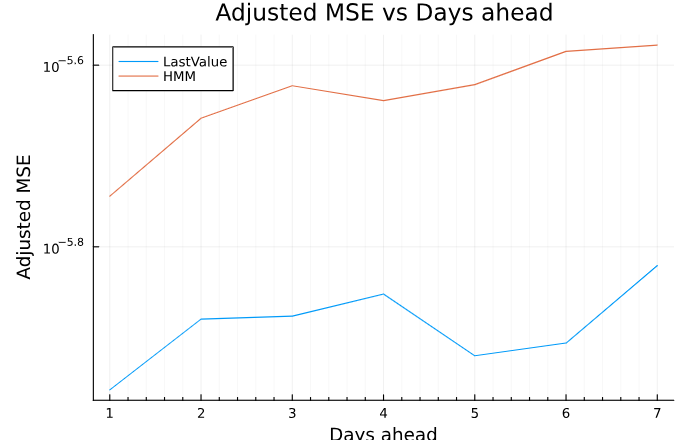
\includegraphics[width=0.7\linewidth]{imgs/ch5/00_raw_comparison_methods.png}
%     \caption{Non tuned variance adjusted comparison between forecasting methods that can produce forecast for the variance }
%     \label{fig:adjustedcomparisonOnlyMu}
% \end{figure}

\clearpage

\section{Backtesting} \label{sec:ch5_backtest}

\subsection{Methodology}

\subsection{Results}
\begin{figure}[ht!]
    \centering
    \includesvg[width=0.7\linewidth]{imgs/ch5/E1_02_BH_Forecast.svg}
    \caption{Portfolio value using Mean-Variance MPC strategy with behavioural forecast.}
    \label{fig:MPC_Behavioural}
\end{figure}

\begin{figure}[ht!]
    \centering
    \includesvg[width=0.7\linewidth]{imgs/ch5/E1_02_LV_Forecast.svg}
    \caption{Portfolio value using Mean-Variance MPC strategy with Last Value forecast.}
    \label{fig:MPC_LV}
\end{figure}

\textbf{Profit optimization parameters:} A second optimization round is performed to compare the result of the forecast error optimization parameters with the optimized profits parameters.

\begin{figure}[ht!]
    \centering
    \includesvg[width=0.7\linewidth]{imgs/ch5/E1_02_BH_Forecast_Optimized.svg}
    \caption{Portfolio value using Mean-Variance MPC strategy with behavioural forecast and profit optimization parameters.}
    \label{fig:MPC_BehaviouralTuned}
\end{figure}

\subsubsection{Benchmarks}


\begin{figure}[ht!]
    \centering
    \includesvg[width=\linewidth]{imgs/ch5/E1_02_best_static_asset_return_all.svg}
    \caption{Returns of all assets.}
    \label{fig:E1_02_best_static_asset_return_all}
\end{figure}

\subsection{Conclusions}

The software for algorithmic trading work, some computational efficiencies can be introduced, particularly for parameter optimization, namely the bottleneck lies on the simulation and lack of gradient descent methods when exploring the parameter space, parallelism can help explore many possibilities simultaneously...


\conclusions % Do not change - required
% EDIT THE CONTENT OF THE FILE
% Conclusions.tex
% You can find it under the folder 
% "chapters" on the left column

% APPENDICES ARE OPTIONAL
% COMMENT OUT BOTH LINES BELOW TO REMOVE THEM
% ADD CHAPTERS TO ADD MULTIPLE APPENDICES
\appendix 
\chapter{Data}

\subsection{NASDAQ Screener August 19 2023.} \label{sec::AppendixNasdaqScreener}

\begin{table}[ht!]
    \centering
    \begin{tabular}{|c|c|c|c|} \hline
    sector                 &   Market Capital  &   symbol &   volume \\\hline
 Industrials            &   1.84693e7  &   AMRS   &    46462130\\
 Industrials            &   2.30754e10 &   KEYS   &     7827145\\
 Industrials            &   1.74133e10 &   CNHI   &     4228176\\
 Industrials            &   2.59578e9  &   PACB   &     3853884\\
 Industrials            &   3.44235e8  &   GEVO   &     2986380\\
 Consumer Discretionary &   6.83964e11 &   TSLA   &   135802827\\
 Consumer Discretionary &   6.19471e9  &   AMC    &    51296838\\
 Consumer Discretionary &   1.37453e12 &   AMZN   &    48469182\\
 Consumer Discretionary &   1.73987e10 &   CCL    &    25667447\\
 Consumer Discretionary &   2.25863e11 &   BABA   &    20391288\\
 Technology             &   2.72802e12 &   AAPL   &    61112270\\
 Technology             &   1.06949e12 &   NVDA   &    58258461\\
 Technology             &   7.25894e11 &   META   &    34173615\\
 Technology             &   1.60714e12 &   GOOGL  &    30491041\\
 Technology             &   2.35137e12 &   MSFT   &    24744801\\
 Real Estate            &   4.14622e9  &   MPW    &    62958612\\
 Real Estate            &   5.74561e9  &   AGNC   &    17479995\\
 Real Estate            &   1.5244e9   &   RLJ    &     8064025\\
 Real Estate            &   1.82702e9  &   OUT    &     3536269\\
 Real Estate            &   2.80685e9  &   ABR    &     3519776\\ 
                        &   1.50228e10 &   CCJ    &     3887189\\
                        &   8.22913e9  &   WRK    &     1777259\\
                        &   8.24339e9  &   WSC    &     1282607\\
                        &   3.08235e10 &   URI    &      712346\\
                        &   8.08151e8  &   EVA    &      682833\\
 \hline
    \end{tabular}
  \caption{NASDAQ screener data on August 19 2023. (1/2)}
    \label{tab:NASDAQ_1}
\end{table}


\begin{table}[ht!]
    \centering
    \begin{tabular}{|c|c|c|c|} \hline
    sector                 &   Market Capital  &   symbol &   volume \\\hline
 Health Care            &   1.86805e8  &   TTOO   &   179030087\\
 Health Care            &   2.42993e6  &   AVTX   &    64116418\\
 Health Care            &   5.57971e8  &   AGEN   &    18047826\\
 Health Care            &   1.366e9    &   GERN   &     7800248\\
 Health Care            &   9.45476e10 &   GILD   &     6483830\\
 Finance                &   1.34113e10 &   CFG    &     6912330\\
 Finance                &   4.86156e9  &   MTG    &     3876200\\
 Finance                &   6.37343e10 &   ICE    &     3858707\\
 Finance                &   1.38711e10 &   SYF    &     3300685\\
 Finance                &   4.68209e10 &   MET    &     3225368\\
 Consumer Staples       &   4.50456e10 &   ABEV   &     6939481\\
 Consumer Staples       &   3.99048e9  &   SFM    &     1580697\\
 Consumer Staples       &   1.12302e9  &   AGRO   &     1067914\\
 Consumer Staples       &   3.00794e9  &   TWNK   &     1021225\\
 Consumer Staples       &   1.69466e10 &   BG     &      999713\\
 Utilities              &   3.88369e10 &   KMI    &    19614882\\
 Utilities              &   9.2358e8   &   INFN   &     2386705\\
 Utilities              &   2.70512e10 &   AWK    &     2192075\\
 Utilities              &   1.89596e10 &   TRGP   &     2068634\\
 Utilities              &   9.18623e8  &   CLNE   &     2002208\\
 Energy                 &   5.20104e9  &   PLUG   &    13153878\\
 Energy                 &   3.20286e10 &   DVN    &     6299212\\
 Energy                 &   8.1374e9   &   AR     &     6291505\\
 Energy                 &   1.06924e10 &   PAA    &     6083728\\
 Energy                 &   3.41401e9  &   KOS    &     3517928\\
 \hline
    \end{tabular}
  \caption{NASDAQ screener data on August 19 2023. (2/2)}
    \label{tab:NASDAQ_2}
\end{table}


% \begin{longtable}[c]{|c|c|c|c|} 
%   \caption{NASDAQ screener data on 19\textsuperscript{th} August 2023.}
%   \label{NASDAQ_Screener}\\
%  % \hline
%  % \multicolumn{4}{| c |}{Begin of Table}\\
%  \hline
%  sector                 &   Market Capital  &   symbol &   volume \\
%  \hline
%  \endfirsthead
 
%  \hline
%  \multicolumn{4}{|c|}{Continuation of Table \ref{NASDAQ_Screener}}\\
%  \hline
%  sector                 &   Market Capital  &   symbol &   volume \\
%  \hline
%  \endhead

%  \hline
%  \endfoot

%  \hline
%  \multicolumn{2}{| c |}{End of Table}\\
%  \hline\hline
%  \endlastfoot
 
% Industrials            &   1.84693e7  &   AMRS   &    46462130\\
%  Industrials            &   2.30754e10 &   KEYS   &     7827145\\
%  Industrials            &   1.74133e10 &   CNHI   &     4228176\\
%  Industrials            &   2.59578e9  &   PACB   &     3853884\\
%  Industrials            &   3.44235e8  &   GEVO   &     2986380\\
%  Consumer Discretionary &   6.83964e11 &   TSLA   &   135802827\\
%  Consumer Discretionary &   6.19471e9  &   AMC    &    51296838\\
%  Consumer Discretionary &   1.37453e12 &   AMZN   &    48469182\\
%  Consumer Discretionary &   1.73987e10 &   CCL    &    25667447\\
%  Consumer Discretionary &   2.25863e11 &   BABA   &    20391288\\
%  Technology             &   2.72802e12 &   AAPL   &    61112270\\
%  Technology             &   1.06949e12 &   NVDA   &    58258461\\
%  Technology             &   7.25894e11 &   META   &    34173615\\
%  Technology             &   1.60714e12 &   GOOGL  &    30491041\\
%  Technology             &   2.35137e12 &   MSFT   &    24744801\\
%  Real Estate            &   4.14622e9  &   MPW    &    62958612\\
%  Real Estate            &   5.74561e9  &   AGNC   &    17479995\\
%  Real Estate            &   1.5244e9   &   RLJ    &     8064025\\
%  Real Estate            &   1.82702e9  &   OUT    &     3536269\\
%  Real Estate            &   2.80685e9  &   ABR    &     3519776\\
%                         &   1.50228e10 &   CCJ    &     3887189\\
%                         &   8.22913e9  &   WRK    &     1777259\\
%                         &   8.24339e9  &   WSC    &     1282607\\
%                         &   3.08235e10 &   URI    &      712346\\
%                         &   8.08151e8  &   EVA    &      682833\\

% \end{longtable}

%\input{AppendixB.tex} % Example second appendix (need to create the file in "chapters")


\cleardoublepage % Do not change - required
\RemoveLabels % Do not change - required
\printbibliography[title={Bibliography},heading=bibintoc] % Do not change - required

\end{document}
